%!TEX encoding = UTF-8 Unicode
\documentclass[a4paper]{compendium}
\usepackage[swedish]{babel}
\addto\captionsswedish{%
  \renewcommand{\appendixname}{Appendix}%
}
%TODO: Glossary
%http://tex.stackexchange.com/questions/5821/creating-a-standalone-glossary/5837#5837

\setlength{\columnsep}{16mm}

\title{
{\vspace{-3cm}\bf\sffamily\Huge\selectfont  Introduktion till programmering med Scala och Java} 
\\ \vspace{1em}%\hspace*{1.5cm}\inputgraphics[width=0.6\textwidth]{../img/gurka} \\
{\sffamily  Grundkurs}\\\vspace{2cm}
%
\includegraphics[height=4cm]{../img/scala-logo.png}
%
\includegraphics[height=4cm]{../img/java-logo.png}
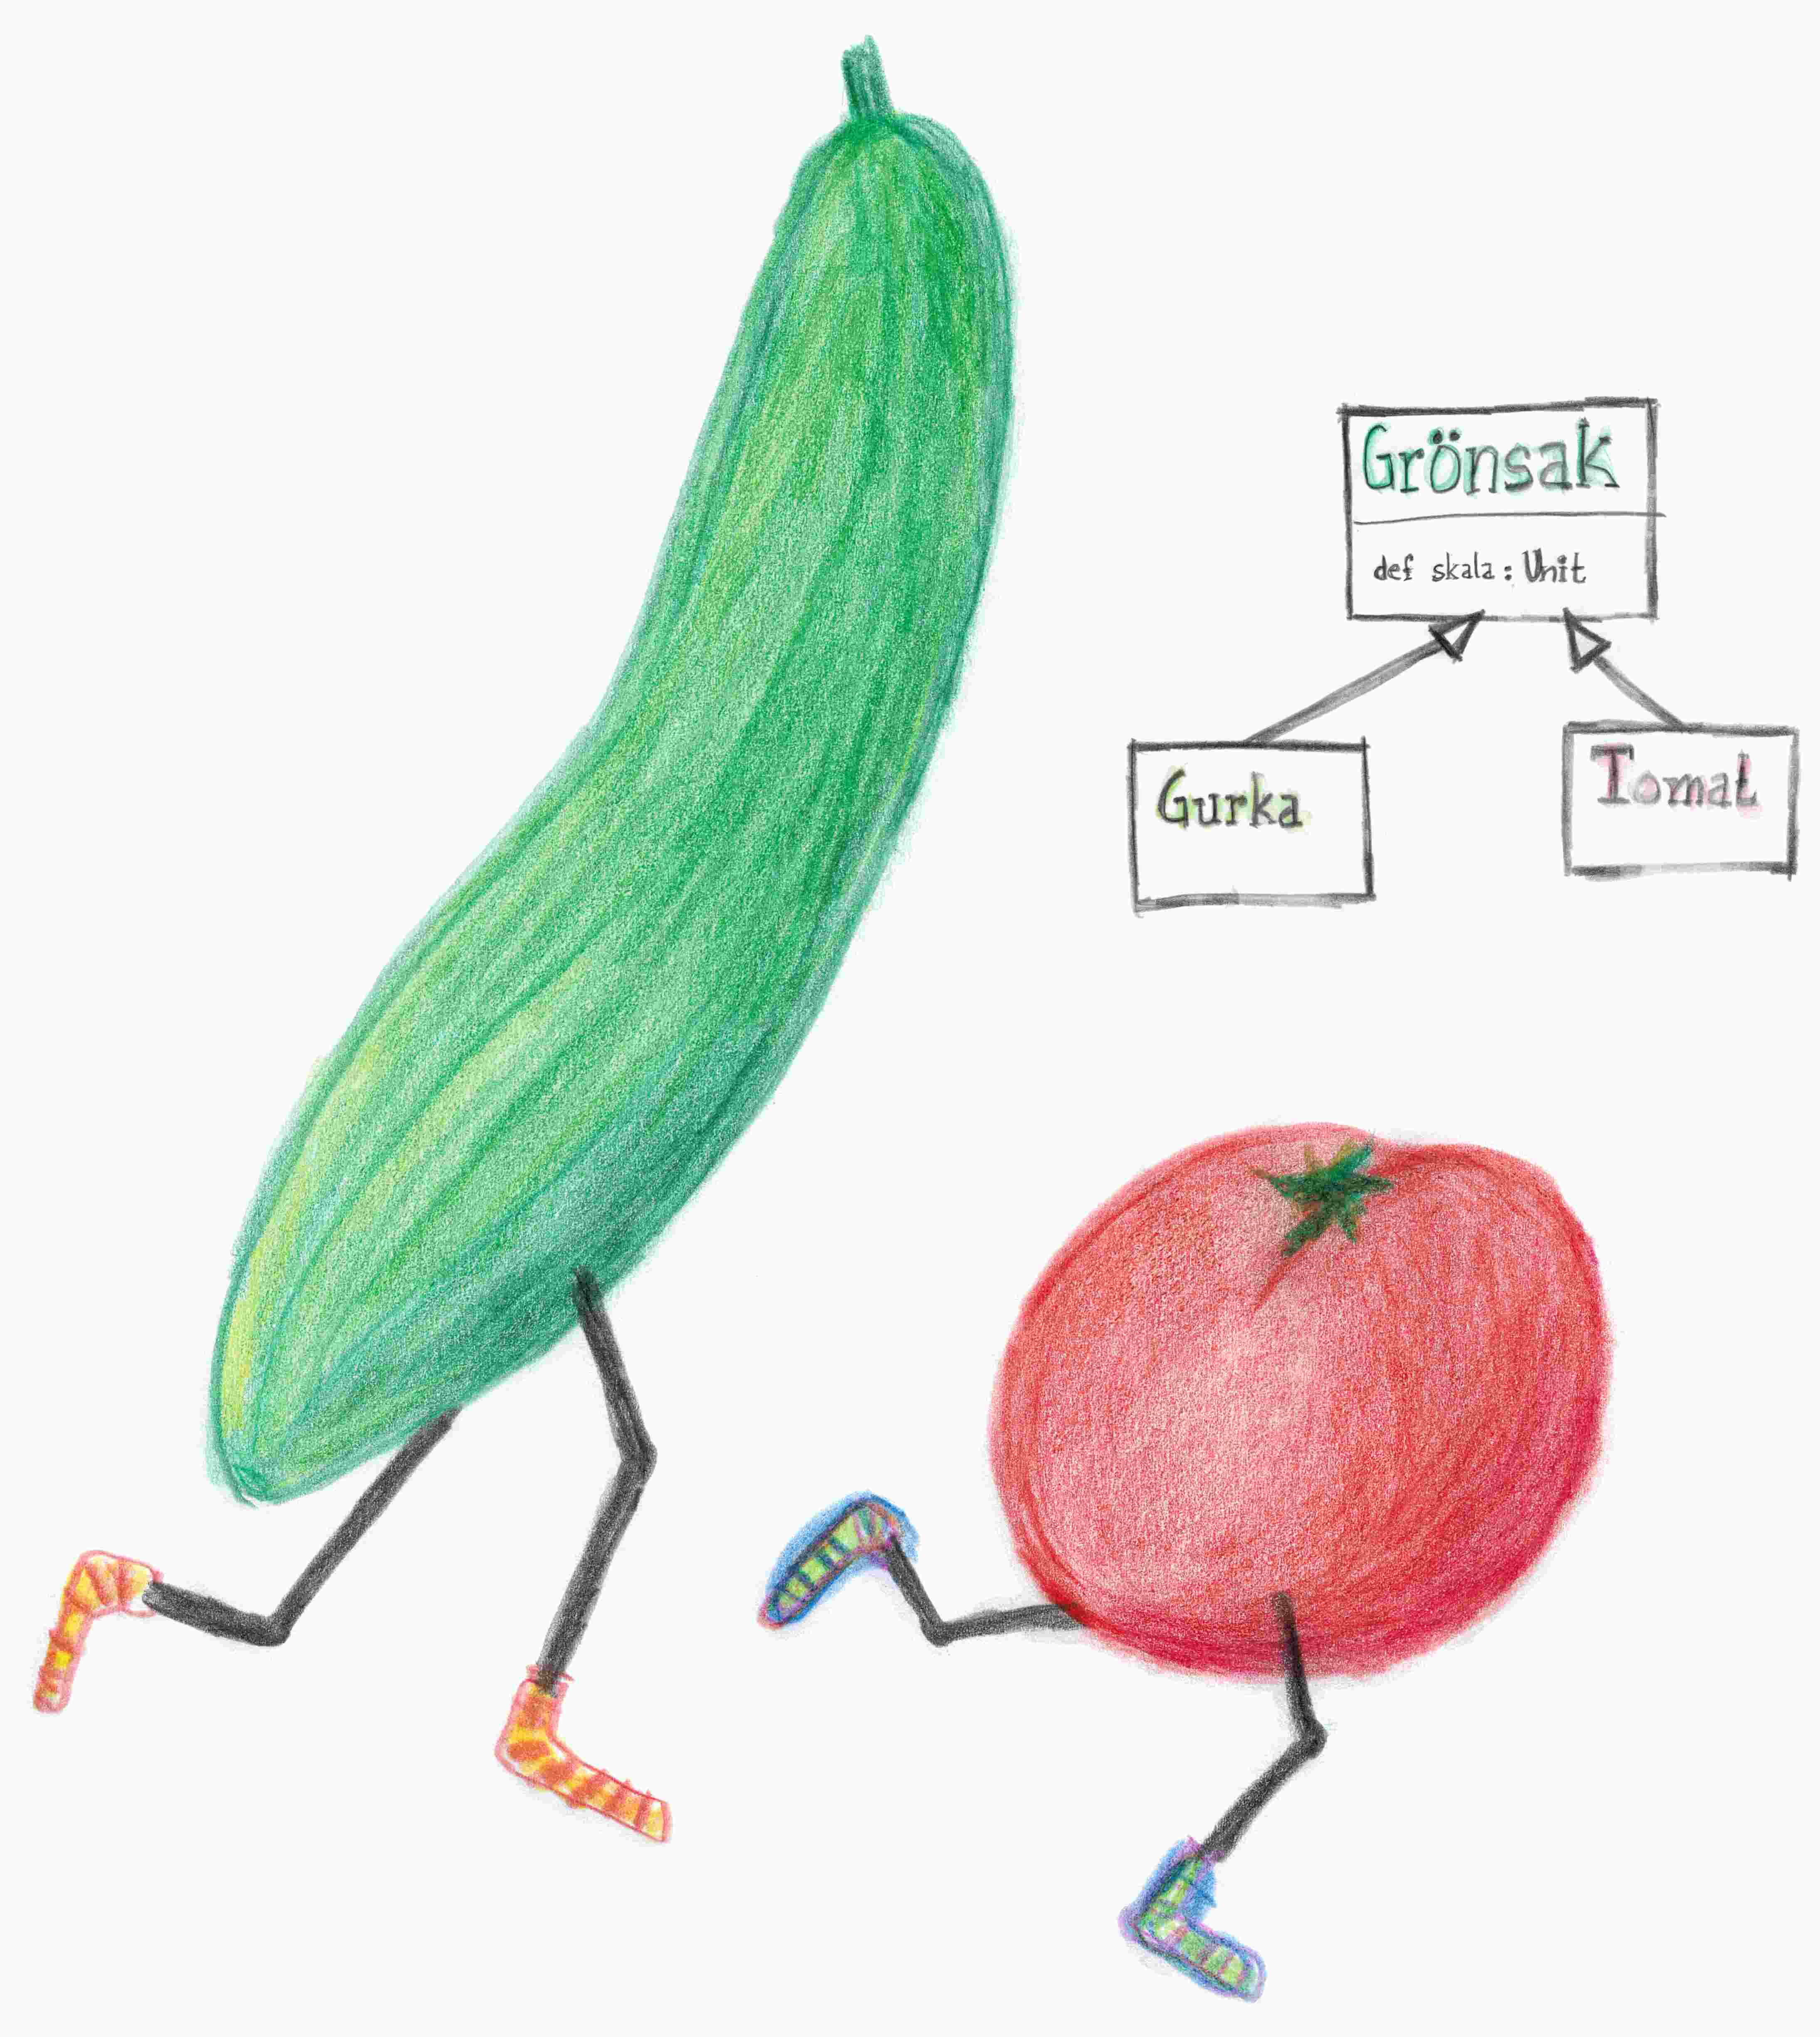
\includegraphics[height=12cm]{cover/gurka.jpg}
}

%\author{Redaktör: Björn Regnell}
\date{EDAA45, Lp1-2, HT 2016 \\ 
Datavetenskap, LTH \\ 
Lunds Universitet  \\~\\ Kompileringsdatum: \today \\
\url{http://cs.lth.se/pgk}
}

\usepackage{pgffor}  %% http://stackoverflow.com/questions/2561791/iteration-in-latex
                     %  allows:  \foreach \n in {1,...,4}{ do something with \n }

\usepackage{framed}  %  allows:   \begin{framed}\end{framed}
%\newenvironment{Slide}[2][]
%  {\begin{framed}\setlist{noitemsep}\section*{#2}}
%  {\end{framed}}

\newcommand{\SlideHeading}[1]{\section*{#1}}

\usepackage[most]{tcolorbox}
\newenvironment{Slide}[2][]
  {\vspace{0.5em}\begin{tcolorbox}[%width=1.05\textwidth,
  grow to right by=0.03\textwidth,grow to left by=0.03\textwidth,%breakable, 
                                   enhanced]\setlist{noitemsep}\SlideHeading{#2}}
  {\end{tcolorbox}\vspace{0.5em}}

\newcommand{\Subsection}[1]{} %ignore slide sections
\newcommand{\SlideOnly}[1]{} %ignore slide font size

\newif\ifkompendium  % to allow conditional text in slides only showing up in compendium
\kompendiumtrue      % in slides: \kompendiumfalse
                

%!TEX encoding = UTF-8 Unicode
\newcommand{\ExeWeekONE}{expressions}
\newcommand{\LabWeekONE}{kojo}

\newcommand{\ExeWeekTWO}{programs}
\newcommand{\LabWeekTWO}{--}

\newcommand{\ExeWeekTHREE}{functions}
\newcommand{\LabWeekTHREE}{bugs}

\newcommand{\ExeWeekFOUR}{data}
\newcommand{\LabWeekFOUR}{pirates}

\newcommand{\ExeWeekFIVE}{sequences}
\newcommand{\LabWeekFIVE}{cards}

\newcommand{\ExeWeekSIX}{classes}
\newcommand{\LabWeekSIX}{turtlegraphics}

\newcommand{\ExeWeekSEVEN}{traits}
\newcommand{\LabWeekSEVEN}{turtlerace-team}

\newcommand{\ExeWeekEIGHT}{matching}
\newcommand{\LabWeekEIGHT}{chords-team}

\newcommand{\ExeWeekNINE}{matrices}
\newcommand{\LabWeekNINE}{maze}

\newcommand{\ExeWeekTEN}{sorting}
\newcommand{\LabWeekTEN}{surveydata-team}

\newcommand{\ExeWeekELEVEN}{scalajava}
\newcommand{\LabWeekELEVEN}{lthopoly-team}

\newcommand{\ExeWeekTWELVE}{threads}
\newcommand{\LabWeekTWELVE}{life}

\newcommand{\ExeWeekTHIRTEEN}{Uppsamling}
\newcommand{\LabWeekTHIRTEEN}{Projekt}

\newcommand{\ExeWeekFOURTEEN}{Extenta}
\newcommand{\LabWeekFOURTEEN}{--}


\begin{document}
\maketitle
%!TEX encoding = UTF-8 Unicode
%!TEX root = ../compendium.tex

\clearpage\null\thispagestyle{empty}
\vfill

{
\setlength{\parindent}{0pt}
\emph{Editor}: Björn Regnell \\ 

\emph{Contributors}: 
Björn Regnell, Erik Bjäreholt, ..., and contributors
\\

\emph{Home}: \url{https://cs.lth.se/pgk} \\ \newline

\emph{Repo}: \url{https://github.com/lunduniversity/introprog} \\ \newline

%\emph{Cover art by}: Poul Ströyer\\ \newline

This manuscript is on-going work. Contributions are welcome! \\ 
\emph{Contact}: \url{bjorn.regnell@cs.lth.se}
\\ \newline

\emph{LICENCE}: CC BY-SA 4.0 \\
\url{http://creativecommons.org/licenses/by-sa/4.0/} \\
Please do \emph{not} distribute your solutions to lab assignments. 
\\ \newline
Copyright \copyright~Computer Science, LTH, Lund University. 2016. Lund. Sweden.\\
}
%!TEX encoding = UTF-8 Unicode
%!TEX root = ../compendium.tex

\ChapterUnnum{Framstegsprotokoll} 


\subsubsection*{Genomförda övningar}

\vspace{1em}\noindent 
{Till varje laboration hör en övning med uppgifter som utgör förberedelse inför labben. Du behöver minst behärska grundövningarna för att klara labben inom rimlig tid. Om du känner att du behöver öva mer på grunderna, gör då även extrauppgifterna. Om du vill fördjupa dig, gör fördjupningsuppgifterna som är på mer avancerad nivå. Kryssa för nedan vilka övningar du har gjort, så blir lätt för din handledare att se vilka kunskaper du förvärvat hittills.}

\newcommand{\TickBox}{\raisebox{-.50ex}{\Large$\square$}}
\newcommand{\ExeRow}[1]{\texttt{#1} & \TickBox  &  \TickBox &  \TickBox  \\ \addlinespace }

\begin{table}[h]
\centering
\vspace{2em}
\begin{tabular}{lccc}
\toprule \addlinespace 
{\sffamily\small Övning} & 
{\sffamily\small Grund} &	
{\sffamily\small Extra} &
{\sffamily\small Fördjupning}\\ \addlinespace \midrule \\[-0.7em]
%!TEX encoding = UTF-8 Unicode
\ExeRow{expressions}
\ExeRow{programs}
\ExeRow{functions}
\ExeRow{data}
\ExeRow{vectors}
\ExeRow{classes}
\ExeRow{traits}
\ExeRow{matching}
\ExeRow{matrices}
\ExeRow{sorting}
\ExeRow{scalajava}
\ExeRow{threads}
\bottomrule
\end{tabular}
\end{table}

\newpage

\subsubsection*{Godkända obligatoriska moment}

\vspace{1em}\noindent 
För att bli godkänd på laborationsuppgifterna och projektuppgiften måste du lösa deluppgifterna och diskutera dina lösningar med en handledare. Denna diskussion är din möjlighet att få feedback på dina lösningar. Ta vara på den!
Se till att handledaren noterar nedan när du blivit godkänd på respektive labb. Spara detta blad tills du fått slutbetyg i kursen. 


\vspace{2.5em}\noindent Namn: \dotfill\\

\vspace{1em}\noindent Namnteckning: \dotfill\\

\newcommand{\LabRow}[1]{\\[-1.1em] \texttt{#1} & \dotfill &  \dotfill  \\ \addlinespace }

\begin{table}[h]
\centering
\vspace{1em}
\begin{tabular}{lcc}
\toprule \addlinespace 
{\sffamily\bfseries\small Lab} & {\sffamily\small Datum gk} &	{\sffamily\small Handledares namnteckning}\\ \addlinespace \midrule \\[-0.5em]
\LabRow{kojo}
\LabRow{simplewindow}
\LabRow{textfiles}
\LabRow{cardgame}
\LabRow{shapes}
\LabRow{turtlerace-team}
\LabRow{newlab-team}
\LabRow{maze}
\LabRow{surveydata-team}
\LabRow{scalajava-team}
\LabRow{life}
\LabRow{Inl.Uppg.}
%\toprule 
\addlinespace \midrule \addlinespace
 \\
{\sffamily\small {\bfseries Projektuppgift} (välj en)	} & \dotfill&\dotfill \\ \addlinespace\addlinespace %\midrule
\texttt{( ) bank}  &  &  \\
\texttt{( ) imageprocessing}  \\
\texttt{( ) tictactoe} \\  
\texttt{( ) }\textit{egendefinerad}  \\
\textit{\small Om egen, ge kort beskrivning:}\\
%\dotfill  \\
\bottomrule
\end{tabular}
\end{table}
%!TEX root = ../compendium.tex


\ChapterUnnum{Förord} 

Programmering är inte bara ett sätt att ta makten över de människoskapade system som är förutsättningen för vårt moderna samhälle. Programmering är också ett kraftfullt verktyg för tanken. Med kunskap i programmeringens grunder kan de som vill påbörja den livslånga läranderesa som det innebär att vara systemutvecklare och abstraktionskonstnär. Programmeringsspråk och utvecklingsverktyg kommer och går, men de grundläggande koncepten bakom \emph{all} mjukvara består: sekvens, alternativ, repetition och abstraktion. 

Detta kompendium utgör kursmaterial för en grundkurs i programmering, som syftar till att ge en solid bas för ingenjörsstudenter och andra som vill utveckla system med mjukvara. Materialet omfattar en termins studier på kvartsfart och förutsätter kunskaper motsvarande gymnasienivå i svenska, matematik och engelska. 

Kompendiet är framtaget för och av studenter och lärare, och distribueras som öppen källkod. Det får användas fritt så länge erkännande ges och eventuella ändringar publiceras under samma licens som ursprungsmaterialet. På kurshemsidan \href{http://cs.lth.se/pgk}{cs.lth.se/pgk} och i kursrepot \href{http://github.com/lunduniversity/introprog}{github.com/lunduniversity/introprog} finns instruktioner om hur du kan bidra till kursmaterialet.

Läromaterialet fokuserar på lärande genom praktiskt programmeringsarbete och innehåller övningar och laborationer som är organiserade i moduler. Varje modul har ett tema och en teoridel i form av föreläsningsbilder med tillhörande anteckningar. 

I kursen använder vi språken Scala och Java för att illustrera grunderna i imperativ och objektorienterad programmering, tillsammans med elementär funktionsprogrammering. Mer avancerad objektorientering och funktionsprogrammering lämnas till efterföljande fördjupningskurser. 

Den kanske viktigaste framgångsfaktorn vid studier i programmering är att bejaka din egen upptäckarglädje och experimentlusta. Det fantastiska med programmering är att dina egna intellektuella konstruktioner faktiskt \emph{gör} något som just \emph{du} har bestämt! Ta vara på det och prova dig fram genom att koda egna idéer -- det är kul när det funkar men minst lika lärorikt är felsökning, buggrättande och alla misslyckade försök som efter hårt arbete vänds till lyckade lösningar och/eller bestående lärdomar. 

Välkommen i programmeringens fascinerande värld och hjärtligt lycka till med dina studier!

\vspace{2em}\noindent\emph{LTH, Lund 2016}



\mainmatter
\tableofcontents

\part{Om kursen}      
%!TEX root = ../compendium.tex

\ChapterUnnum{Kursens arkitektur}
\begin{framed}
\noindent\resizebox{\columnwidth}{!}{%
\begin{tabular}{l|l|l|l|l|l|l}
\textit{W} & \textit{Datum} & \textit{Lp V} & \textit{Modul} & \textit{Förel} & \textit{Övn} & \textit{Lab} \\ \hline \hline
W01 & 29/8-2/9    & Lp1V1 & Introduktion         & F01 F02 & expressions & kojoturtle      \\
W02 & 5/9-9/9     & Lp1V2 & Kodstrukturer        & F03 F04 & programs    & --              \\
W03 & 12/9-16/9   & Lp1V3 & Funktioner, Objekt   & F05 F06 & functions   & simplewindow    \\
W04 & 19/9-23/9   & Lp1V4 & Datastrukturer       & F07 F08 & data        & textfiles       \\
W05 & 26/9-30/9   & Lp1V5 & Vektoralgoritmer     & F09 F10 & vectors     & cardgame        \\
W06 & 3/10-7/10   & Lp1V6 & Klasser, Likhet      & F11 F12 & classes     & shapes          \\
W07 & 10/10-14/10 & Lp1V7 & Arv, Gränssnitt      & F13 F14 & traits      & turtlerace-team \\
KS  & ksdatum     & TP1   & KONTROLLSKRIVN.      & --      & --          & --              \\
W08 & 31/10-4/11  & Lp2V1 & Mönster, Undantag    & F15 F16 & matching    & newlab-team     \\
W09 & 7/11-11/11  & Lp2V2 & Matriser             & F17 F18 & matrices    & maze            \\
W10 & 14/11-18/11 & Lp2V3 & Sökning, Sortering   & F19 F20 & sorting     & surveydata-team \\
W11 & 21/11-25/11 & Lp2V4 & Scala och Java       & F21 F22 & scalajava   & scalajava-team  \\
W12 & 28/11-2/12  & Lp2V5 & Trådar, Web, Android & F23 F24 & threads     & life            \\
W13 & 5/12-9/12   & Lp2V6 & Design               & F25 F26 & Uppsamling  & Inl.Uppg.       \\
W14 & 12/12-16/12 & Lp2V7 & Tentaträning         & F27 F28 & Extenta     & --              \\
T   & tentadatum  & TP2   & TENTAMEN             & --      & --          & --              \\
\end{tabular}

}
\end{framed}
\newcommand{\Subsection}[1]{} %ignore slide sections

\newenvironment{Slide}[2][]
  {\begin{framed}\setlist{noitemsep}\section*{#2}}
  {\end{framed}}

\newif\ifkompendium
\kompendiumtrue

%!TEX root = ../lect-week01.tex

%%%%%%%%%%%%%%%%%%%%%%%%%%%%%%%%%%%%%%
\Subsection{Om denna kurs}

%%%
\begin{Slide}{Vad och hur?}
\begin{itemize}
\item \emph{Vad} ska du lära dig?
\begin{itemize}
\item Grundläggande principer för programmering\\ $\implies$Inga förkunskaper i programmering krävs!
\item Konstruktion av (enkla) algoritmer
\item Tänka i abstraktioner
\item Imperativ och objektorienterad programmering
\item Programspråket Java
\item Utvecklingsmiljön Eclipse: implementera, testa, felsöka
\end{itemize}

\item \emph{Hur} ska du lära dig?
\begin{itemize}
\item Genom praktiskt eget arbete: \Emph{Lära genom att göra!}
\item Genom studier av kursens teori: \Emph{Skapa förståelse!}
\item Genom samarbete med dina kurskamrater: \Emph{Gå djupare!}
\end{itemize}
\end{itemize}
\end{Slide}


\ifkompendium
\subsection{hej}
Denna text hamnar bara i kompediet

Hejsan svejsan

\begin{itemize}
\item some item
\end{itemize}


\begin{Code}
hej kod
\end{Code}
\fi


\ifkompendium\else
\begin{Slide}{TESTSLAJD EJ I KOMPENDIUM}
\begin{itemize}
\item \emph{Hej} på dig
\item blablab
\item blabla
\end{itemize}
\begin{Code}
hej kod
\end{Code}
\end{Slide}
\fi


%%%%%%%%%%%%%%%%%%%%%%%%%%%%%%%%%%%%%%
\ifkompendium\else
\Subsection{Meddelande från \href{http://lth.se/code}{Code@LTH}} 
\fi

\begin{itemize}
\item item
\item item
\item item
\item item
\end{itemize}


%!TEX root = ../compendium.tex

\ChapterUnnum{Anvisningar}

\SectionUnnum{Samarbetsgrupper}
\subsection*{Samarbetskontrakt}
\SectionUnnum{Föreläsningar}
\SectionUnnum{Övningar}
\SectionUnnum{Laborationer}
\SectionUnnum{Resurstider}
\SectionUnnum{Kontrollskrivning}
\SectionUnnum{Tentamen}


\renewcommand{\SlideHeading}[1]{\section{#1}}

\part{Moduler}         
\foreach \n in {1,...,9}{%
  \input{modules/w0\n-chapter.tex} 
  \input{modules/w0\n-exercise.tex}
  \input{modules/w0\n-lab.tex}
}
\foreach \n in {10,...,12}{%
  \input{modules/w\n-chapter.tex} 
  \input{modules/w\n-exercise.tex}
  \input{modules/w\n-lab.tex}
}

%!TEX root = ../compendium.tex

%!TEX encoding = UTF-8 Unicode
\chapter{Design}\label{chapter:W13}
Koncept du ska lära dig denna vecka:
\begin{multicols}{2}\begin{itemize}[nosep,label={$\square$},leftmargin=*]
\item\end{itemize}\end{multicols}

    
%!TEX encoding = UTF-8 Unicode
%!TEX root = ../compendium.tex

\Assignment{bank}

\begin{Goals}
\item Kunna implementera ett helt program efter given specifikation
\item Förstå hur Java-klasser kan användas i Scala
\item Förstå och bedöma när immutable/mutable såväl som var/val bör användas i större sammanhang
\item Kunna använda sig av kompanjons-objekt
\item Kunna läsa och skriva till fil
\item Kunna söka i olika datastrukturer på olika sätt
\end{Goals}

\subsection{Bakgrund}

I denna uppgiften ska du skriva ett program som håller reda på bankkonton och kunder i en bank. Programmet ska även hålla reda på bankens nuvarande tillstånd, såväl som föregående.
Tillstånden ska vid varje tillståndsförändringar skrivas till fil så att utifall banken skulle krascha finns alla transaktioner som genomförts sparade så att banken kan återställas.

Programmet ska vara helt textbaserat, man ska alltså interagera med programmet via konsollen där en meny skrivs ut och input görs via tangentbordet.

Du ska skriva hela programmet själv, men det ska dock följa de specifikationer som ges i uppgiften, såväl som de objektorienterade principer du lärt dig i kursen.

\subsection{Krav}

Kraven för bankapplikationen återfinns här nedan. För att bli godkänd på denna uppgift måste samtliga krav uppfyllas:

\begin{itemize}
\item Programmet ska ha följande funktioner tillgängliga via menyn:

\begin{itemize}
\item Hitta konton för en viss kontoinnehavare.
\item Sök kontoinnehavare på (del av) namn.
\item Sätta in pengar på ett konto.
\item Ta ut pengar på ett konto.
\item Överföra pengar mellan två olika konton.
\item Skapa ett nytt konto.
\item Ta bort ett befintligt konto.
\item Skriv ut bankens alla konton.
\item Återställa banken till ett tidigare tillstånd vid ett givet datum.
\item Avsluta.
\end{itemize}

\item Programmet ska skapa nytt tillstånd med tidsstämpel och spara gamla varje gång då:
\begin{itemize}
\item Pengar sätts in eller tas ut ifrån ett konto.
\item Pengar överförs mellan två konton.
\item Ett konto skapas.
\item Ett konto tas bort.
\end{itemize}
\item Då ett tillstånd förändras ska detta skrivas till fil.
\item Programdesignen ska följa de specifikationer som är angivna nedan.
\item Inga utskrifter eller inläsningar får göras i klasserna Customer, BankAccount, Bank, State eller Transaction. Allt som berör användargränssnittet ska ske i BankApplication. Det är tillåtet att använda valfritt antalat hjälpmetoder och hjälpklasser i klassen BankApplication.
\item Alla metoder och attribut ska ha lämpliga åtkomsträttigheter.
\item Valet av val/var och immutable/mutable måste vara lämpliga.
\item Din indata måste ge samma resultat som i exemplen (som kommer komma i framtiden) i bilagan.
\item Rimlig felhantering ska finnas, det är alltså önskvärt att programmet inte kraschar då man matar in felaktig input, utan istället säger till användaren att input är ogiltlig.

\end{itemize}

\subsection{Design}
Nedan följer specifikationerna för de olika klasserna bankapplikationen måste innehålla:

BankAccount

\begin{Code}
/**
 * Skaper ett nytt bankkonto åt innehavaren Customer.
 * Kontot tilldelas ett unikt kontonummer och innehåller 
 * inledningsvis 0 kr.
 */
class BankAccount(val holder: Customer);

  /**
   * Sätter in mängden amount pengar på detta konto.
   */
  def deposit(amount: Int): Unit;

  /**
   * Hämtar saldot på konton.
   */
  def getBalance: Int;

/**
   * Tar ut mängden amount pengar från kontot sålänge
   * amount ej överstiger nuvarande saldo.
   * Returnerar true om transactionen lyckades, annars false. 
   */
  def withdraw(amount: Int): Boolean;

\end{Code}

Bank

\begin{Code}
/**
 * Skapar en ny bank utan konton och tillstånd. 
 */
class Bank();

/**
   * Skapar ett nytt konto på banken. Kontonumret som 
   * genereras åt kontot returneras.
   */
  def addAccount(name: String, id: Int): Int

/**
   * Returnerar kontoinnehavaren kopplat till det givna 
   * id-numret, om ingen sådan kund finns returneras 
   * null istället.
   */
  def findHolder(id: Int): Customer;

/**
   * Ta bort kontot med kontonumret accountNbr och returnerar
   * true. 
   * Om inget sådant konto existerar returneras false istället. 
   */
  def removeAccount(accountNbr: Int): Boolean;

/**
   * Returnerar en lista med samtliga bankkontot i banken.
   * Finns inga kontot returneras en tom lista.
   */
  def getAllAccounts(): ArrayBuffer[BankAccount];

/**
   * Returnerar det bankkonto som har kontonummer accountNbr.
   * Finns inget sådant konto returneras null istället.
   */
  def findByNumber(accountNbr: Int): BankAccount;

/**
   * Söker upp alla konton med en innehavaren vars namn 
   * innehåller strängen namePattern och returnerar dessa
   *  i en lista.
   */
  def findByName(namePattern: String): ArrayBuffer[Customer];

/**
   * Genomför en transaktioner i banken och returnerar en sträng 
   * med nödvändig information till konsolen.
   */
  def makeTransaction(transaction: Transaction): String;

/**
   * Återställer banken till det tillstånd som gällde vid
   * tiden date.
   */
  def returnToState(returnDate: Date): String;


\end{Code}

Transaction

\begin{Code}
/**
 * Beskriver en transaktion som används av banken.
 */
abstract class Transaction;

\end{Code}


Customer

\begin{Code}
/**
 * Beskriver en kund med namnet name och personnummer id.
 */
class Customer(val name: String, val id: Int);

\end{Code}



\subsection{Obligatoriska uppgifter}

\Task Skapa klassen BankApplication.

\Subtask Klassen BankApplication ska innehålla main-metoden. Det kan vara bra att innan man fortsätter se till att denna klass skriver ut menyn korrekt och kan ta input från tangentbordet.

\Task Skapa klassen Bank.

\Task Skapa klassen Customer.

\Task Skapa klassen BankAccount.

\Task Skapa de klasser som förlängar Transaction

\Task För att ge transaktioner och tillstånd en tidsstämpel ska en wrapper av java.time användas

\begin{Code}
/** A simple wrapper of Java.time */
case class Date;
\end{Code}

\subsection{Frivilliga extrauppgifter}

\Task Ej bestämt ännu.


%!TEX encoding = UTF-8 Unicode
%!TEX root = ../compendium.tex

\Assignment{tictactoe}

\begin{Goals}
	\item Implementera ett helt program efter specifikation.
	\item Få en inblick i hur rekursion kan användas, utöver svans-rekursion.
	\item Bli introducerad till spelteori och hur man kan uttrycka optimal strategi för spelet tictactoe.
	\item Träna på att använda abstrakta klasser.
	\item Kunna byta mellan representationer av en spelplan.
\end{Goals}

I detta projektet ska du implementera din egen version av spelet tic-tac-toe (eller som vi på svenska kallar det, tre i rad)! Du kommer börja med att implementera en version där du kan spela mot en kursare och sen gå vidare till att implementera en datorspelare som lägger sin pjäs slumpmässigt och till slut en som inte kan förlora!

\subsection{Regler}
Om du känner dig säker på hur reglerna i tic-tac-toe funkar kan du skippa detta. 
\begin{itemize}
	\item Spelplanen består av ett rutnät av storlek 3x3.
	\item Det finns två spelare: \texttt{x} och \texttt{o}.
	\item Spelarna placerar ut en pjäs var i växlande ordning där \texttt{x} börjar.
	\item Spelet tar slut om en spelare har fått antingen en rad, diagonal eller kolumn ifylld av sin spelpjäs eller om spelplanen är fylld.
\end{itemize}
\textit{Notera att pjäserna INTE får flyttas när de väl ligger på spelplanen.}

\subsection{Teori}
Representationen är vald till en endimensionell vektor av typen Int av storlek 9 där element $[0,2]$ \footnote{med beteckningen [x,y] menas alla heltal från x till y, dvs: x, x+1, x+2, ... , y-1, y. [0,2] = {0,1,2}} representerar den första raden $[3,5]$ andra och $[6,8]$ den tredje. Anledningen till detta är att vi vill ha en representation så att spelaren kan svara vilket drag den vill göra med ett heltal.
Varje element i vektorn ska kunna representera en tom plats, en plats allokerad av \texttt{x} och en plats allokerad av \texttt{o}. Detta innebär att en vektor av typen Boolean inte räcker till. Istället väjs den (kanske lite minnesöverflödiga) typen Int. Vi har valt representationen där 0 representerar tom plats, 1 representerar \texttt{x} och -1 representerar \texttt{o}. Denna representation är dels smidig för vår framtida OptimalP och även för att avgöra om spelare \texttt{x} eller \texttt{o} har vunnit. Man kan exempelvis summera en rad och kolla om radens summa är 3, då har \texttt{x} vunnit eller -3, då har \texttt{o} vunnit.
 
\subsection{Obligatoriska uppgifter}

\Task Implementera ett fungerande Spel.

\Subtask Implementera funktionen gameWon.

\Subtask Implementera en HumanP.

\Subtask Implementera en version av Game, börja med att alltid spela ett spel och alltid rita spelplanen. main, draw och play behöver implementeras. Men all funktionalitet i main behöver ännu inte finnas.\footnote{Notera att man behöver invertera spelplanen om den ska skickas till spelare två (alternativs låta spelaren hålla reda på om den är \texttt{x} eller \texttt{o}). Förslagsvis löses detta med en extra funktion invGame som skapar en ny array med omvända tecken till orginalarrayen.}

\Task Randomized player

\Subtask Skapa en ny utökning av Player (kopiera HumanP, och byt namn till RandP) där move istället för att läsa från System.in väljer ett random giltigt drag.

\Subtask Ändra Game så att användaren tillåts stänga av ritfunktionen och i så fall tillåts välja antalet spel.

\Subtask Vad är sannolikheterna för att \texttt{x} vinner, \texttt{o} vinner och att det blir oavgjort om två randomized players spelar mot varandra?

Hamnar man i närheten av dessa resultat tror vi på er RandP.
\begin{itemize}
	\item P(\texttt{x} vinner) = 0.586
	\item P(\texttt{o} vinner) = 0.288
	\item P(lika) = 0.126
\end{itemize}

\Subtask Varför är det större sannolikhet för \texttt{x} att vinna än \texttt{o}?

\Task Optimal Player

Betrakta den givna funktionen \texttt{eval}
\begin{Code}
/* returns 1 if there is a guaranteed strategy for who to win 
 * returns 0 if there is a guaranteed strategy for who to draw 
 * returns -1 if the opponent can force a win,
 * no matter what who does.
 * This is done by min,max-evaluation. 
 * Find the move that gives the oppoent the worst possible
 * position and return -min, this is our max.
 */
def eval(game: Array[Int], depth: Int, who: Int): Int = {
	if(gameWon(game,-who)) return -1;
	if(depth == 9) return 0;
	var min = 1;
	for(i <- 0 until 9) {
		if(game(i) == 0) {
			game(i) = who;
			val score = eval(game,depth+1,-who);
			if(score<min){
				min = score;
			}
			game(i) = 0;
		}
	}
	-min;
}
\end{Code}

\texttt{eval} avgör om du är i en vinnande, förlorande eller oavgjord situation, givet att båda spelare spelar optimalt. Det som nog är svårast att förstå är varför vi retunerar \texttt{-min} på slutet. \texttt{min} sparar det sämsta värdet som vår motståndare kan få givet våra möjliga drag. Vi observerar att vi är i precis omvänd situation jämfört med vår motståndare. Om vår moståndare definitivt vinner förlorar vi definitivt, om det blir oavgjort för vår motståndare blir det också oavgjort för oss, och om vår motståndare definitivt förlorar, då vinner vi. Vi representerade ju vinst med 1, oavgjort med 0 och förlust med -1. Det är alltså härifrån minustecknet kommer ifrån. Vill man läsa mer om detta kan man kolla in wikipedias artikel https://en.wikipedia.org/wiki/Minimax om minmax-evaluering. Vi tar helt enekelt det draget som är sämst för vår motståndare.

\Subtask Implementera move-funktionen till OptimalP.

\Subtask Låt två OptimalP spela mot varandra några gånger (10-typ). Det skall alltid bli oavgjort.

\Subtask Testa att spela mot din OptimalP med en HumanP. Kan du spela lika? Kan du vinna?

\Subtask Vad händer om du sätter en RandP mot OptimalP? Blir det någonsin oavgjort, hur ofta? Bilr det någon skillad man byter vem som får spela först.

\Task Säkerhet

I nuläget finns det förmodligen ett problem med din nuvarande implemntation, och det är att du skickar iväg en mutable datastruktur till en Player som utifrån den mutable datan skall göra ett drag. Tänk om en elak programmerare bestämmer sig för att ändra på spelplanen i sin egna players move-metod. Då skulle man i princip kunna fuska. För att lösa detta kan man skicka en kopia till spelaren från Game.

\subsection{Frivilliga extrauppgifter}

\Task Hashning.

Om du låter en OptimalP spela mot en RandP 1000 gånger lär det ta ganska lång tid. Det behöver det inte göra. När OptimalP bestämmer vilket drag den skall göra första gången går den ju igenom alla andra möjliga drag man kan komma till. Det visar sig att det inte finns så många unika spelbräden. Färre än $3^9 < 20000$. Sparar man ett värde till varje sådant spelbräde i en HashMap kan man bara fråga HashMapen vilket drag som är bäst givet ett spelbräde. Detta går väldigt snabbt, jämfört med ungefär $9! > 300000$ funktionsanrop för ett drag på ett tomt spelbräde. Således behöver vi bara gå igenom våra evauleringsmetoder en gång för att bygga hashmapen, sedan går det jättesnabbt för vår HashOptimalP att spela tictactoe. 

Man får dock vara lite klurig, en Array[Int] går inte att använda som key i en hashMap, då den inte har en implementerad hashCode-funktion. Enklast är att göra om vår array till en sträng, genom att lägga värdena i arrayen efter varandra i strängen. Vi kan göra en privat funktion \texttt{hash(Array[Int]):String} som konkatenerar värdena i arrayen. hash([0,0,0,1,1,0,-1,-1,0]) skall alltså retunera "000110-1-10".

\Subtask Skapa en ny subklass HashOptimalP.

\Subtask Skapa och implementera en privat metod \texttt{hash(Array[Int]):String}

\Subtask Implementera en konstruktor som skapar och genererar en HashMap.

Här kan du använda koden som används i evalfunktionen, men du måste komma ihåg att innan du retunerar måste ett key-value-par läggas in i din hashmap.

\Subtask Låt move-funktion göra en hashlookup med hjälp av hash-funktionen och din HashMap.

\Subtask Testa att låta två HashOptimalP spela mot varandra. Du märker nog att skapandet av en sådan spelare kommer ta lite tid, typ en halv sekund. Sedan skall det dock gå jättesnabbt när spelarna spelar. 100000 spel skall gå utan problem på någon sekund, vilket borde gå på tiotals minuter för den gamla OptimalP.
%!TEX encoding = UTF-8 Unicode
%!TEX root = ../compendium.tex

\Assignment{imageprocessing}

\subsection{Bakgrund}

En digital bild består av ett rutnät (en matris) av pixlar. Varje pixel har en färg, och om man har många pixlar flyter de samman för ögat så att de tillsammans skapar en bild.

Det finns olika system för hur man färgsätter de olika pixlarna. T.ex. så används CMYK-systemet (cyan, magenta, gul, svart) vid blandning av färg som ska tryckas på papper eller annat material. På en dator däremot används vanligtvis RGB-systemet. RGB-systemet har tre grundfärger: röd, grön och blå. Mättnaden av varje grundfärg anges av ett heltal som vi i fortsättningen förutsätter ligger i intervallet [0, 255]. 0 anger ”ingen färg” och 255 anger ”maximal färg”. Man kan därmed representera 256 × 256 × 256 = 16 777 216 olika färgnyanser. Man kan också representera gråskalor; det gör man med färger som har samma värde på alla tre grundfärgerna: (0, 0, 0) är helt svart, (255, 255, 255) är helt vitt.


\subsection{Uppgiften}
Du ska skriva ett program där du implementerar olika filter som ska manipulera en given bild på ett flertal olika sätt. Filterklasserna ska ärva från en abstrakt \code{ImageFilter}-klass som är skriven i Java.

Följande beskriver \code{ImageFilter}-klassen.

\begin{JavaSpec}{abstract class ImageFilter}
/**
 * Skapar ett filterobjekt med ett givet namn.
 */
protected ImageFilter(String name);

/**
 * Tar reda på filtrets namn.
 */
public String getName();

/**
 * Filtrerar bilden i matrisen inPixels och returnerar
 * resultatet i en ny matris. Utnyttjar eventuellt 
 * värdet av paramValue
 */
public abstract Color[][] apply(Color[][] inPixels,
				 double paramValue);

/**
 * Berättar huruvida ett filter behöver ett parmetervärde eller inte
 * @return true ifall parametervärde behövs, annars false
 */
public abstract boolean needsParameter();

/**
 * Beräknar intensiteten hos alla pixlarna i pixels,
 * returnerar resultatet i en ny matris.
 */
protected short[][] computeIntensity(Color[][] pixels):

/**
 * Faltar punkten p[i][j] med faltningskärnan kernel.
 * 
 * @param p 		matris med talvärden
 * @param i 		radindex får den aktuella punkten
 * @param j 		kolonnindex får den aktuella punkten
 * @param kernel	faltningskärnan, en 3x3-matris
 * @param weight	summan av elementen i kernel
 * @return 		resultatet av faltningen
 */
protected short convolve(short[][] p, int i, int j, 
			short[][] kernel, int weight);
\end{JavaSpec}

Utöver filterklasserna ska du även implementera \code{FilterChooser} som hanterar val av filter och \code{FilterList} som kan applicera ett variabelt antal filter på en och samma bild. Du får tillgång till en \code{Image}-klass som representerar en bild samt ett \code{ImageUI} som hjälper att ladda in en JPEG bild.

\begin{ScalaSpec}{Image}
class Image(val image: BufferedImage);

/** Returns a matrix of Color-objects that represents an image */
def getColorMatrix: Array[Array[Color]];

/** Updates the image in accordance with the given Color-matrix */
def updateImage(pixels: Array[Array[Color]]): Unit;
\end{ScalaSpec}

\begin{ScalaSpec}{FilterList}
class FilterList = ???

/** Adds a filter to the FilterList */
def addFilter(filter: ImageFilter): Unit = ???
  
/** Applies all the filters on the given Image and draws it in SimpleWindow */
def applyFilters(image: Image, sw: SimpleWindow): Unit = ???
\end{ScalaSpec}

\begin{ScalaSpec}{FilterChooser}
/** Creates a FilterChooser with all the available filters */
class FilterChooser(filters: Array[ImageFilter]) = ???
  
/** Shows which filters are available and lets the user choose filters
*   until an escape sequence has been given and returns a FilterList which
*   contain the chosen filters
*   Example: 
*   Tryck på 1 för Blått-filter
*   Tryck på 2 för Kontrast-filter
*   Tryck på 3 för Gauss-filter
*   Tryck på 4 för Sobel-filter
*   Tryck 42 om du inte vill ha fler filter
*/
def chooseFilters(): FilterList = ???
\end{ScalaSpec}


\Task Implementera ett blåfilter. Det vill säga skapa ett filter där varje pixelelement bara innehåller den blå komponenten. Testa filtret genom att skriva en main metod. Använd \code{ImageUI} för att välja en bild på följande sätt:
\begin{Code}
val im = new Image(ImageUI.getImage)
\end{Code}
Använd \code{SimpleWindow} för att visa bilden.

\Task Implementera ett inverteringsfilter som skapar en negativ kopia av bilden. 
Fundera över vad som kan menas med en inverterad eller negativ kopia: de nya RGB-värdena är inte ett dividerat med de gamla värdena (då skulle de nya värdena kunna bli flyttal) och inte de gamla värdena med ombytt tecken (då skulle de nya värdena bli negativa).

\Task Implementera ett filter som gör om bilden till en gråskalebild. Använd \code{ImageFilter}s \code{computeIntensity} metod för att bestämma vilken intensitet varje bildelement ska ha. Om intensiteten i ett bildelement till exempel är 105 så ska ett nytt \code{Color}-objekt med värdena (105, 105, 105) skapas.

\Task Skapa ett filter som krypterar bilden med xor-operatorn. Varje bildelement krypteras genom att använda xor-operatorn med ursprungsvärdena för rött, grönt och blått tillsammans med ett slumpmässigt heltalsvärde som genereras av Javas Random klass.

\Task Gaussfiltrering. Skriv en klass \code{GaussFilter} där \code{ImageFilter}s \code{convolve}-metod används. Varje färg ska behandlas separat. Gör på följande sätt:
\begin{enumerate}
	\item Bilda tre short-matriser och lagra pixlarnas red-, green- och blue-komponenter i matriserna.
	\item Utför faltningen av de tre komponenterna för varje element och lagra ett nytt \code{Color}-objekt i \code{outPixels} för varje punkt.
	\item Elementen i ramen behandlas inte, men i \code{outPixels} måste också dessa element få värden. Enklast är att flytta över dessa element oförändrade från \code{inPixels} till \code{outPixels}. Man kan också sätta dem till \code{Color.WHITE}, men då kommer den filtrerade bilden att se något mindre ut.
\end{enumerate}

Metoden faltar punkten p[i][j] med faltningskärnan \code{kernel} och ska anropas med red-, green- och blue-matrisen. \code{weight} är summan av elementen i \code{kernel}. Faltningskärnan kan vara ett attribut i klassen och ska vara en matris med följande utseende:
$$
\begin{pmatrix}
  0 & 1 & 0 \\
  1 & 4 & 1 \\
  0 & 1 & 0 \\
\end{pmatrix}
$$
\Task Sobelfiltrering.
\begin{enumerate} 
	\item Beräkna intensitetsmatrisen med metoden \code{computeIntensity}.
	\item Falta varje punkt i intensitetsmatrisen med två kärnor:
$$
X\_SOBEL =
\begin{pmatrix}
  -1 & 0 & 1 \\
  -2 & 0 & 2 \\
  -1 & 0 & 1 \\
\end{pmatrix}
Y\_SOBEL =
\begin{pmatrix}
  -1 & -2 & -1 \\
  0 & 0 & 0 \\
  1 & 2 & 1 \\
\end{pmatrix}
$$
	Använd metoden \code{convolve} med vikten 1. Koefficienterna i matrisen $X\_SOBEL$ uttrycker derivering i x-led, i $Y\_SOBEL$ faltning i y-led. För att förklara varför koefficienterna ibland är 1 och ibland 2 måste man studera den bakomliggande teorin noggrant, men det gör vi inte här.
	\item Om resultaten av faltningen i en punkt betecknas med $sx$ och $sy$ så får man en indikator på närvaron av en kontur med $Math.abs(sx) + Math.abs(sy)$. Absolutbelopp behöver man eftersom man har negativa koefficienter i faltningsmatriserna. 
	\item  Sätt pixeln till svart om indikatorn är större än tröskelvärdet, till vit annars. Tröskelvärdet bestäms av \code{paramValue}. Skriv en klass \code{SobelFilter} som implementerar denna algoritm.
\end{enumerate}

\Task Implementera \code{FilterList} enligt specifikationerna ovan.

\Task Implementera \code{FilterChooser} enligt specifikationerna ovan.

\Task Knyt ihop allt i ett \code{ImageProcessing}-object som ska innehålla en \code{main}-metod där allt körs från. Utskrifterna ska se ut på följande sätt:

{\setlength{\parindent}{0cm}

 Välj en av följande bilder genom att mata in en siffra\newline

0. boy.jpg\newline
1. car.jpg\newline
2. duck.jpg\newline
3. facade.jpg\newline
4. jay.jpg\newline
5. moon.jpg\newline
6. obidos.jpg\newline
7. sgrada.jpg\newline
8. shuttle.jpg\newline
Ditt val: 1\newline
Bild car.jpg laddad\newline
Tryck på 0 för Vanligt-filter\newline
Tryck på 1 för Blått-filter\newline
Tryck på 2 för Krypterat-filter\newline
Tryck på 3 för Inverterat-filter\newline
Tryck på 4 för Grått-filter\newline
Tryck på 5 för Kontrast-filter\newline
Tryck på 6 för Gauss-filter\newline
Tryck på 7 för Sobel-filter\newline
Tryck 42 om du inte vill använda fler filter\newline
Välj ett filter 1\newline
Välj ett filter 42\newline
Välja ny bild? (y/n) n\newline
}

Tänk på att användaren kan mata in otillåtna värden. Detta ska hanteras på lämpligt sätt.

\subsection{Frivilliga extrauppgifter}

\Task Förbättring av kontrasten i bild. Vi inskränker oss här till att förbättra kontrasten i gråskalebilder. Om man applicerar kontrastfiltrering på en färgbild så kommer bilden att konverteras till en gråskalebild. (Man kan naturligtvis förbättra kontrasten i en färgbild och få en färgbild som resultat. Då behandlar man de tre färgkanalerna var för sig.) Många bilder lider av alltför låg kontrast. Det beror på att bilden inte utnyttjar hela det tillgängliga området 0–255 för intensiteten. Man får en bild med bättre kontrast om man ”töjer ut” intervallet enligt följande formel (lineär interpolation):

$$newIntensity = 255 * (intensity - 45) / (225 - 45)$$

Som synes kommer en punkt med intensiteten 45 att få den nya intensiteten 0 och en punkt med intensiteten 225 att få den nya intensiteten 255. Mellanliggande punkter sprids ut jämnt över intervallet $[0, 255]$. För punkter med en intensitet mindre än 45 sätter man den nya intensiteten till 0, för punkter med en intensitet större än 225 sätter man den nya intensiteten till 255. Vi kallar intervallet där de flesta pixlarna finns för \code{[lowCut, highCut]}. De punkter som har intensitet mindre än \code{lowCut} sätter man till 0, de som har intensitet större än \code{highCut} sätter man till 255. För de övriga punkterna interpolerar man med formeln ovan (45 ersätts med \code{lowCut}, 225 med \code{highCut}).

Det återstår nu att hitta lämpliga värden på \code{lowCut} och \code{highCut}. Detta är inte något som kan göras helt automatiskt, eftersom värdena beror på intensitetsfördelningen hos bildpunkterna. Man börjar med att beräkna bildens intensitetshistogram, dvs hur många punkter i bilden som har intensiteten 0, hur många som har intensiteten 1, . . . , till och med 255. Detta är ett typiskt registreringsproblem som ska lösas enligt metoden i avsnitt 8.10 i läroboken. %Kanske ändra och förklara då Per Holms bok inte ska användas?

I de flesta bildbehandlingsprogram kan man sedan titta på histogrammet och interaktivt bestämma värdena på \code{lowCut} och \code{highCut}. Så ska vi dock inte göra här. I stället bestämmer vi oss för ett procenttal \code{cutOff} (som vi matar in i Parameter-rutan i användargränssnittet) och beräknar \code{lowCut} så att \code{cutOff} procent av punkterna i bilden har en intensitet som är mindre än \code{lowCut} och \code{highCut} så att \code{cutOff} procent av punkterna har en intensitet som är större än \code{highCut}.

Exempel: antag att en bild innehåller 100 000 pixlar och att \code{cutOff} är 1.5. Beräkna bildens intensitetshistogram i en vektor $int[] histogram = new int[256]$. Beräkna \code{lowCut} så att $histogram[0] + histogram[1] + ... + histogram[lowCut] = 0.015 * 100000$ (så nära det går att komma, det blir troligen inte exakt likhet). Beräkna \code{highCut} på liknande sätt.
Sammanfattning av algoritmen:
\begin{enumerate}
	\item Beräkna intensiteten hos alla punkterna i bilden, lagra dem i en \code{short}-matris. Använd den färdigskrivna metoden \code{computeIntensity}.
	\item Beräkna bildens intensitetshistogram.
	\item Parametervärdet \code{paramValue} är det värde som ska användas som \code{cutOff}.
	\item Beräkna \code{lowCut} och \code{highCut} enligt ovan.
	\item Beräkna den nya intensiteten för varje pixel enligt interpolationsformeln och lagra de nya pixlarna i \code{outPixels}.
\end{enumerate}
Skriv en klass \code{ContrastFilter} som implementerar algoritmen. I katalogen \emph{images} kan bilden \emph{moon.jpg} vara lämpliga att testa, eftersom den har låg kontrast. Anmärkning: om \code{cutOff} sätts = 0 så får man samma resultat av denna filtrering som man får av \code{GrayScaleFilter}. Detta kan man se genom att studera interpolationsformeln.

%!TEX encoding = UTF-8 Unicode

%!TEX root = ../compendium.tex

\chapter{Tentaträning}\label{chapter:W14}
\begin{multicols}{2}\begin{itemize}[nosep,label={$\square$}]
\item\end{itemize}\end{multicols}


%!TEX encoding = UTF-8 Unicode
%!TEX root = ../lect-week14.tex

%%%

\Subsection{Tentatips}
\begin{Slide}{Före tentan:}\footnotesize
\begin{enumerate}
\item Repetera övningar och labbar i kompendiet. 
\item Läs igenom föreläsningsanteckningar.
\item Studera \Emph{snabbref} \Alert{mycket noga} så att du vet vad som är givet och var det står, så att du kan hitta det du behöver snabbt.
\item Skapa och \Emph{memorera} en personlig \Emph{checklista} med programmeringsfel du brukar göra, som även inkluderar småfel, så som glömda parenteser och semikolon, och annat som en kompilator/IDE normalt hittar.
\item Tänk igenom hur du ska disponera dina 5 timmar på tentan.
\item Gör den fiktiva extentan som om det vore \Alert{skarpt läge}: 
\begin{enumerate}\footnotesize
\item Avsätt 5 ostörda timmar (stäng av telefon, dator etc).
\item Inga hjälpmedel. Bara snabbref.
\item Förbered dryck och tilltugg.
\end{enumerate}
\end{enumerate}
\end{Slide}

\begin{Slide}{På tentan:} \footnotesize
\begin{enumerate}
\item Läs igenom \Alert{hela} tentan först. \\ \Emph{Varför?} Förstå helheten. Delarna hänger ihop.
\item Notera och begrunda specifika begrepp och definitioner. \\ \Emph{Varför?} Begreppen är avgörande för förståelsen av uppgiften.
\item Notera förenklingar, antaganden och specialfall. \\ \Emph{Varför?} Uppgiften blir mkt enklare om du inte behöver hantera dessa.
\item \Alert{Fråga} tentamensansvarig om du inte förstår uppgiften -- speciellt om det finns misstänkta felaktigheter eller förmodat oavsiktliga oklarheter. \\ \Emph{Varför?} Det är inte lätt att konstruera en ''perfekt'' tenta. \\ Du får fråga vad du vill, men det är inte säkert du får svar :)
\item Läs specifikationskommentarerna och metodsignaturerna i alla givna klass-specifikationer \Alert{mycket noga}. \\ \Emph{Varför?} Det är ett vanligt misstag att förbise de ledtrådar som ges där.
\item Återskapa din memorerade personliga checklista för vanliga fel som du brukar göra och avsätt tid till att gå igenom den på tentan.
\item Lämna in ett försök även om du vet att lösningen inte är fullständig. 
\end{enumerate}
\end{Slide}

     


\part{Appendix}         
\appendix
%!TEX encoding = UTF-8 Unicode
%!TEX root = ../compendium.tex

\chapter{Terminalfönster}\label{appendix:terminal}

\section{Vad är ett terminalfönster?}

I ett terminalfönster kan man skriva kommandon som kör program och hanterar filer. När man programmerar använder man ofta terminalkommando för att kompilera och exekvera sina program.  
 
\subsubsection{Terminal i Linux}

    \begin{figure}[!b]
    \centering
    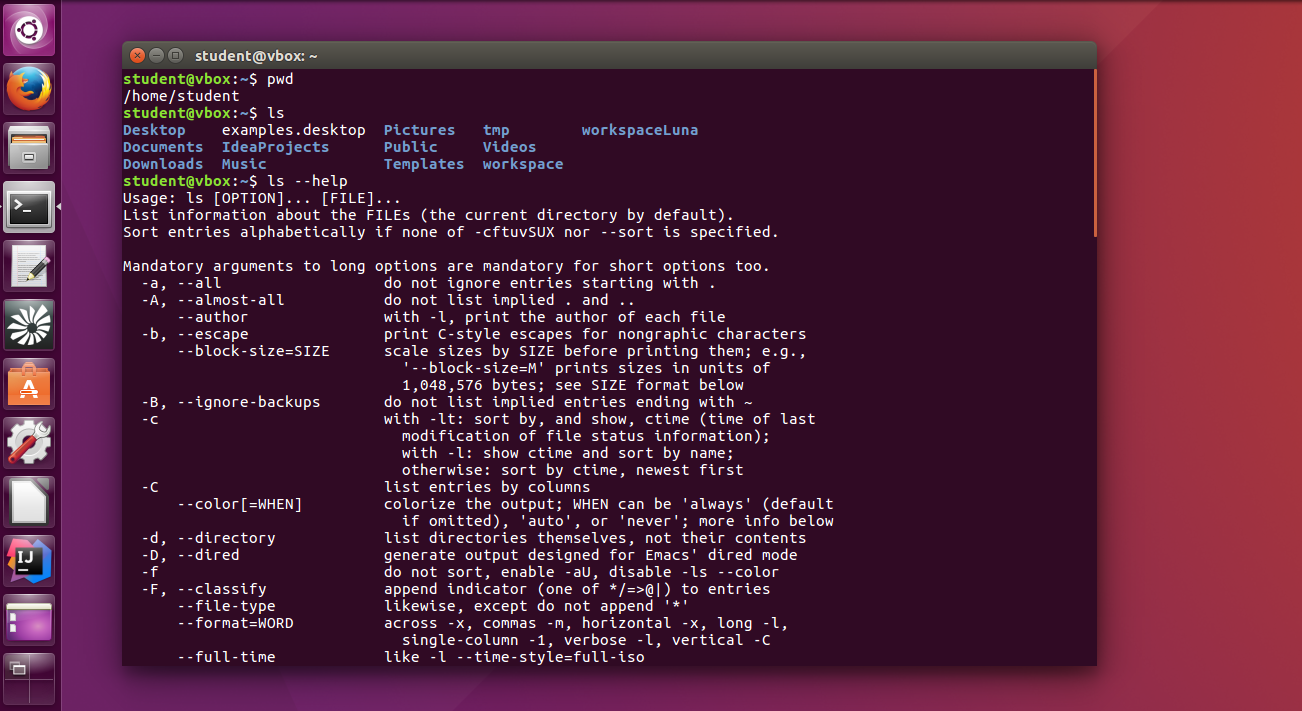
\includegraphics[width=1.0\textwidth]{../img/linux-terminal.png}
    \caption{Terminalfönster i Ubuntu öppnas med Ctrl+Alt+T.}
    \label{fig:terminal:linux}
    \end{figure}

I Ubuntu trycker du lättast \textbf{Ctrl+Alt+T} eller sök efter ''terminal'' i app-menyn.  Då öppnas ett fönster med en blinkande markör som visar att det är redo att ta emot dina textkommando. Ett exempel på kommando är \texttt{ls} som skriver ut en lista med filer i det aktuella biblioteket, så som visas i fig. \ref{fig:terminal:linux}.

Det som visas i ett terminalfönster sköts av ett \textbf{kommandoskal} \Eng{command shell}, som är redo att ta emot kommando efter en prompt som slutar med ett \texttt{\$}-tecken. När du skriver ett kommando och trycker Enter anropar kommandoskalet en kommandotolk som tolkar och utför dina kommandon. Om ett kommando inte kan tolkas, skrivs ett felmeddelande. 

Det finns många användbara kortkommando, varav de viktigaste visas i tabell \ref{fig:terminal:shortcuts}. Det är bra om du lär dig dessa kortkommandon utantill så att ditt arbete i terminalen går snabbt och smidigt.

\begin{table}[H]
\renewcommand{\arraystretch}{1.15}
\begin{tabular}{@{}r | l}
pil upp/ner & bläddra i kommandohistoriken \\
Tab & ''auto-complete'', fyll i resten baserat på vad du skrivit hittills \\
Tab Tab & två tryck på Tab listar flera alternativ, om så finnes \\
Ctrl+A & ''ahead'', flytta markören till början av raden \\
Ctrl+E & ''end'', flytta markören till slutet av raden \\
Ctrl+K & ''kill'', ta bort tecken från markören till radens slut\\
Ctrl+U & ''undo'', ta bort tecken från markören till början av raden \\
Ctrl+Y & ''yank'', sätt in det som senast togs bort\\
Ctrl+Z & ''zleep'', stoppa pågående process, skriv sedan \texttt{bg} för bakgrundskörning\\
Ctrl+L & rensa terminalfönstret\\
Ctrl+D & avsluta kommandoskalet \\
\end{tabular}
    \caption{Viktiga kortkommandon i Linux terminalfönster.}
    \label{fig:terminal:shortcuts}
\end{table}

\noindent Ctrl+C orsakar normalt ett avbrott av pågående process, men om du vill att Ctrl+C ska vara ''Copy'' som vanligt för att kopiera markerad text, kan du ställa om detta med terminalförnstrets  meny ''Edit $\rightarrow$ Keyboard Shortcuts'', eller liknande.




 
\subsubsection{PowerShell och Cmd i Microsoft Windows}
Microsoft Windows är inte Linux-baserat, men i kommandotolken \textbf{Powershell} finns alias definierade för några vanliga Linux-kommandon, inkluderat \texttt{ls}, \texttt{cd} och \texttt{pwd}. 
Du startar Powershell t.ex. genom att trycka på Windows-knappen och skriva \texttt{powershell}. 
Du kan också, medan du bläddrar bland filer, klicka på filnamnsraden överst i filbläddraren och skriva \texttt{powershell} och tryck Enter; då startas Powershell i aktuellt bibliotek. Ändra gärna typsnitt och bakgrundsfärg med hjälp av fönstrets menyer, så att det blir lättare för dig att läsa vad som skrivs.

Det finns även i Windows den ursprungliga kommandotolken \textbf{Cmd} med helt andra kommandon. Till exempel skriver man i Cmd kommandot \texttt{dir} i stället för \texttt{ls} för att lista filer. 

I Windows 10 du även köra Ubuntu-kommandoskalet, se\\ \href{http://www.omgubuntu.co.uk/2016/08/enable-bash-windows-10-anniversary-update}{http://www.omgubuntu.co.uk/2016/08/enable-bash-windows-10-anniversary-update}



\subsubsection{Terminal i Apple OS X / macOS}


Apple OS X och macOS är Unix-baserade operativsystem. De flesta vanliga terminalkommandon som fungerar i Linux fungerar också under Apple OS X och macOS. Du startar ett terminalfönster i Apples operativsystem genom att klicka på förstoringsglaset uppe till höger, skriva \texttt{terminal}, och trycka Enter.

\section{Vad är en path/sökväg?}\label{terminal:path}

När du skriver ett kommando i terminalen, eller kör vilket program som helst på din dator, behöver operativsystemet identifera i vilken fil programmets maskinkod ligger innan programmet kan köras. 

Lokaliseringe av filer sker med hjälp av en \textbf{sökväg} \Eng{path}, som anger en position i filsystemet. Ofta betraktas filsystemet som ett upp-och-ned-vänt träd, och kallas därför även ''filträdet''. Den ''översta'' positionen kallas ''rot'' \Eng{root} och betecknas med ett enkelt snedstreck \texttt{/}. Kataloger som ligger i kataloger utgör förgreningar i trädet. En sökväg pekar ut vägar genom trädet som behövs för att nå ''löven'', som utgörs av själva filerna.

Du kan se var ett program ligger i Linux med hjälp av kommandot \texttt{which} enligt nedan.\footnote{Skriv \texttt{ gcm ls } i Windows Powershell för motsvarighet till \texttt{ which ls } \\ Eller skriv \texttt{ New-Alias which get-command } för tillgång till kommandot \texttt{which} i Powershell. \\ \href{http://stackoverflow.com/questions/63805/equivalent-of-nix-which-command-in-powershell}{stackoverflow.com/questions/63805/equivalent-of-nix-which-command-in-powershell}} Listan med bibliotek i sökvägen avskiljs med snedstreck.
\begin{REPLnonum}
$ which java
/usr/lib/jvm/oracle_jdk8/bin/java
$ which ls
/bin/ls
\end{REPLnonum}

En sökväg kan vara \textbf{absolut} eller \textbf{relativ}. En absolut sökväg utgår från roten och visar hela vägen från rot till destination, t.ex. \texttt{/usr/bin/firefox}, medan en relativ sökväg utgår från aktuellt bibliotek (där du ''står'') och börjar \textit{inte} med ett snedstreck.

Alla operativsystem håller reda på en mängd olika sökvägar för att kunna hitta speciella filer i filträdet. Dessa sökvägar lagras i s.k. \textbf{miljövariabler} \Eng{environment variables}. Det finns en \textit{speciell} miljövariabel som heter kort och gott \textbf{PATH}, i vilken alla sökvägar till de program finns, som ska vara tillgängliga för din användaridentitet direkt för exekvering genom sina filnamn, \textit{utan} att man behöver ange absoluta sökvägar. 

Du kan i Linux se vad som ligger i din PATH med kommandot \code{ echo $PATH } medan man i Windows Powershell skriver \code{$env.Path} där det bara är första bokstaven som ska vara en versal. I Lunix separeras biblioteken i sökvägen med kolon, medan Windows använder semikolon.

Ibland kan du behöva uppdatera din PATH för att program som du installerat och ska bli allmänt tillgängliga. Detta görs på lite olika sätt i olika operativsystem, för Linux se t.ex. här:
\href{http://stackoverflow.com/questions/14637979/how-to-permanently-set-path-on-linux}{stackoverflow.com/questions/14637979/how-to-permanently-set-path-on-linux}

När man anger sökvägar finns några tecken med speciell betydelse:

\begin{tabular}{r  p{0.8\textwidth}}
\code|~| & ''tilde'', din hemkatalog \\
\code|/| & ''slash'', snedstreck anger filträdets rot om det finns i början av sökvägen, men utgör biblioteksavskiljare inuti sökvägen \\
\code|.| & en punkt anger aktuellt bibliotek, där du ''står'' \\
\code|..| & två punkter anger ett steg ''upp'' i filträdet \\
\code|"| & omgärda en sökväg med citationstecken, först och sist, om den innehåller annat än engelska bokstäver, t.ex. blanktecken\\
\code|\ | & \textit{backslash+blanktecken} används för att beteckna mellanslag i sökvägar som \textit{inte} omgärdas av citationstecken\\
\end{tabular}

\section{Några viktiga terminalkommando}

I tabell \ref{fig:terminal:commands} finns en lista med några viktiga terminalkommando som är bra att lära sig utantill.

En introduktion till LTH:s datorer med exempel på hur du använder vanliga Linux-kommandon finns i denna skrift \url{http://www.ddg.lth.se/perf/unix/} som används i introduktionsveckan för nybörjare på datateknikprogrammet vid LTH.

På sajten \url{http://ss64.com/} finns en mer omfattande lista med användbara terminalkommando och tillhörande förklaringarför för Linux (Bash), Windows (Powershell, Cmd) och Apple OS X.  

\begin{table}[H]
\renewcommand{\arraystretch}{1.25}
   
\begin{tabular}{@{}r | l}
\texttt{ls} & lista filer i aktuellt bibliotek (alltså där du ''står'')\\
\texttt{ls} \textit{p}  & lista filer i biblioteket  \textit{p} \\
\texttt{ls -A} & lista alla filer i aktuellt bibliotek, även gömda \\
\texttt{man ls} & manual för kommandot \texttt{ls}; testa även \texttt{man} för andra kommandon! \\
\texttt{cd} \textit{p} & ''change directory'', ändra aktuellt bibliotek till \textit{p}\\
\texttt{pwd} & ''print working directory'', skriv ut sökväg för aktuellt bibliotek \\
\texttt{cp} \textit{p1 p2} & ''copy'', kopiera filen med path \textit{p1} till en ny fil kallad \textit{p2} \\
\texttt{mv} \textit{p1 p2} & ''move'', byt namn på filen \textit{p1} till \textit{p2}  \\
\texttt{rm} \textit{p} & ''remove'', ta bort filen \textit{p}\\
\texttt{rm -r} \textit{p} & ''remove recursive'', ta bort biblioteket \textit{p} med allt innehåll; var försiktig!\\
\texttt{mkdir} \textit{p} & ''make dir'', skapa ett nytt bibliotek \textit{p}\\
\texttt{cat} \textit{p1 p2}& ''concatenate'', skriv ut hela innehållet i en eller flera filer \textit{p1 p2 etc.}\\
\texttt{less} \textit{p}& skriv ut innehållet i filen \textit{p}, en skärm i taget\\
\texttt{wget} \textit{url}&ladda ner \textit{url}, t.ex. \texttt{ wget http://cs.lth.se/pgk/ws -o ws.zip}\\
\texttt{unzip} \textit{p}& packa upp \textit{p}, t.ex. \texttt{ unzip ws.zip}\\
\end{tabular}

    \caption{Några viktiga terminalkommando i Linux. Med \textit{p}, \textit{p1}, \textit{p2}, etc.  avses en absolut eller relativ sökväg \Eng{path}, se avsnitt \ref{terminal:path}.}
    \label{fig:terminal:commands}

\end{table}


%!TEX encoding = UTF-8 Unicode
%!TEX root = ../compendium.tex

\chapter{Editera}\label{appendix:edit}
\section{Vad är en editor?}

En editor används för att redigera programkod. Det finns många olika editorer att välja på. Erfarna utvecklare lägger ofta mycket energi på att lära sig att använda favoriteditorns kortkommandon och specialfunktioner, eftersom detta påverkar stort hur snabbt kodredigeringen kan göras. 

En bra editor har \textbf{syntaxfärgning} för språket du använder, så att olika delar av koden visas i olika färger. Då går det mycket lättare att läsa och hitta i koden. 

Nedan listas några viktiga funktioner som man använder många gånger dagligen när man kodar:

\begin{itemize}
\item \textbf{Navigera}. Det finns flera olika sätt att flytta markören och bläddra genom koden. Alla editorer erbjuder sökmöjligheter, och de flesta editorer har även mer avancerade sökfunktioner där kodmönster kan identifieras och multipla sökträffar markeras över flera kodfiler. 

\item \textbf{Markera}. Att markera kod kan göras på många sätt: med piltangenter+Shift, med olika speciella menyalternativ, med mus + dubbelklick eller trippelklick, etc. I vissa editorer finns även möjlighet att ha multipla markörer så att flera rader kan editeras samtidigt.

\item \textbf{Kopiera}. Genom Copy-Paste slipper du du skriva samma sak många gånger. Kortkommandona Ctrl+C för Copy och Ctrl+V för Paste sitter i fingrarna efter ett tag. Man ska dock vara medveten om att det lätt blir fel när man kopierar en stor del som sedan ska ändras lite; många Copy-Paste-buggar kommer av att man inte är tillräckligt noggrann och ofta är det bättre att skriva från grunden i stället för att kopiera så att du hinner tänka efter medan du skriver.

\item \textbf{Klipp ut}. Genom Ctrl+X för Cut och Ctrl+V för Paste, kan du lätt flytta kod. Att skriva kod är en stegvis process där man gör många förändringar under resans gång för att förbättra och vidareutveckla koden. Att flytta på kod för att skapa en bättre struktur är mycket vanligt.

\item \textbf{Formatering}. Med indragningar, radbrytningar och nästlade block i flera nivåer får koden struktur. Många editorer kan hjälpa till med detta och har speciella kortkommandon för att ändra indragningsnivå inåt eller utåt. 

\item \textbf{Parentesmatchning}. Olika former av parenteser, \code+ ( { [ ) } ] +,  behöver matchas för att koden ska fungera; annars går kompilatorn ofta helt vilse och konstiga felmeddelanden kan peka på helt fel plats i koden. En bra kodeditor kan hjälpa dig att markera vilka parentespar som hör ihop så att du undviker att spendera för mycket tid med att leta efter en parentes som saknas eller är står i vägen.
    
\end{itemize}

I en integrerad utvecklingsmiljö, en s.k. IDE, (se appendix \ref{appendix:ide}) finns en inbyggd editor som, tack vare ett mer intimt samarbete med kompilatorn, kan erbjuda ännu fler avancerade funktioner som hjälper dig i kodarbetet. Men även när du lärt dig använda en IDE kommer du fortfarande ha stor nytta av en ''vanlig'' editor. Ofta har man flera terminalfönster igång, tillsammans med flera editorfönster och en IDE. 

\section{Välj editor}

I tabell \ref{edit:popular-editors} visas en lista med några populära editorer. Det är en stor fördel om din favoriteditor finns på flera plattformar så att du har nytta av dina förvärvade färdigheter när du behöver växla mellan olika operativsystem. 

Om du inte vet vilken du ska välja, börja med \textit{gedit}, som inte är så avancerad, men därför lätt att komma igång med. När du sedan är redo att investera din lärotid i en mer avancerad editor rekommenderas \textit{Atom}, eftersom den är öppen, gratis och finns för Linux, Windows och macOS. 

Det är är också bra att lära sig åtminstone de mest basala kommandona i editorn \textit{vim} eftersom denna  editor kan köras direkt i terminalen, även vid fjärrinloggning, och finns förinstallerad i de flesta Linux-system.


\begin{table}[T]

\renewcommand{\arraystretch}{1.25}

\begin{tabular}{@{}r | p{0.75\textwidth}}
\textit{Editor} & \textit{Beskrivning} \\ \hline

Gedit & öppen, fri och gratis; lätt att lära men inte så avancerad; finns för Linux, Windows \& macOS; är förinstallerad på LTH:s Linux-datorer och startas med kommandot \verb+gedit+ i ett terminalfönster; skriven i C och Python \newline  
 \url{https://wiki.gnome.org/Apps/Gedit} \\

Atom & öppen, fri och gratis; finns för Linux, Windows, \& macOS; är förinstallerad på LTH:s Linux-datorer och startas med kommandot \verb+atom+ i ett terminalfönster; utvecklingen startades nyligen av GitHub och därför är Atom ännu inte lika mogen som övriga editorer i denna lista; skriven i Javascript och Coffeescript och exekverar under  Electron med hjälp av Chromium och Node.js \newline \url{https://atom.io/} \\

Vim & öppen, fri och gratis; lång historik, hög inlärningströskel; finns för Linux, Windows, \& Mac; är förinstallerad på LTH:s Linux-datorer och startas med kommandot \verb+vim+ i ett terminalfönster; skriven i C \newline \url{http://www.vim.org/} \\

Emacs & öppen, fri och gratis; lång historik, hög inlärningströskel; finns för Linux, Windows, \& Mac; är förinstallerad på LTH:s Linux-datorer och startas med kommandot \verb+emacs+ i ett terminalfönster; skriven i Lisp och C \newline \url{http://www.gnu.org/software/emacs/} \\

Sublime Text 3 & stängd kod; gratis att prova på, men programmet föreslår då och då att du köper en licens;  skriven i C++ och Python; finns för Windows, Mac, Linux. \newline
 \url{http://www.sublimetext.com/3} \\


Notepad++ & öppen, fri och gratis; finns endast för Windows; skriven i C++, \url{https://notepad-plus-plus.org/} \\


Textwrangler & stängd kod, gratis; lätt att lära men inte så avancerad; finns endast för macOS  
\newline \url{http://www.barebones.com/products/textwrangler/} \\

\end{tabular}
    \caption{Några populära editorer. Om du inte vet vilken du ska välja, börja med att installera Gedit.}
    \label{edit:popular-editors}
\end{table}
%!TEX root = ../compendium.tex

\chapter{Kompilera och exekvera}\label{appendix:compile}
\section{Vad är en kompilator?}
\section{Java JDK}
\subsection{Installera Java JDK}
\section{Scala}
\subsection{Installera Scala-kompilatorn}
\section{Read-Evaluate-Print-Loop (REPL)}
För många språk, t.ex. Scala och Python, finns det en interaktiv tolk som gör det möjligt att exekvera enstaka programrader och direkt se effekte. En sådan tolk kallas Read-Evaluate-Print-Loop eftersom den läser en rad i taget och översätter till maskinkod som körs direkt.    
\subsection{Scala REPL}
\subsubsection{Kommandon i REPL}
:paste

Kortkommandon: Ctrl+K etc.
%!TEX encoding = UTF-8 Unicode
%!TEX root = ../compendium.tex

\chapter{Dokumentation}\label{appendix:doc}

Dokumentation hjälper andra att använda din kod, men underlättar även för dig själv när du vid ett senare tillfälle ska erinra dig hur den fungerar och hur du ska använda och bygga vidare på din kod. Modern systemutveckling baseras ofta på öppen källkod och färdiga api \Eng{application programming interface}, där kvaliteten på dokumentationen är avgörande för hur lätt det är att komma igång med att använda koden.

Nedan listas exempel på olika typer av  dokumentation\footnote{\href{https://en.wikipedia.org/wiki/Software_documentation}{en.wikipedia.org/wiki/Software\_documentation}}:

\begin{itemize}
\item \textbf{Kravdokumentation} beskriver det övergripande målet med mjukvaran, samt funktionella krav och kvalitetskrav som uppfylls av systemet.
\item \textbf{Designdokumentation} beskriver arkitekturen, hur koden är organiserad i moduler, och den interna systemstrukturen t.ex. i form av klasser, objekt och deras relation.
\item \textbf{Slutanvändardokumentation} kan t.ex. vara manualer för användning av systemet och installationsanvisningar.
\item \textbf{Teknisk dokumentation} kan t.ex. vara api-dokumentation som beskriver vilka funktioner som ingår i ett programbibliotek. Sådan dokumentation genereras ofta med hjälp av ett \textbf{dokumentationsverktyg} (se avsnitt \ref{appendix:buildtool}).  Andra typer av teknisk dokumentation är instruktioner om hur man bygger koden med eventuellt tillhörande byggverktygskonfigurationsfiler; ofta beskrivs byggförfarandet steg för steg i en textfil med namnet \code{README}. (Läs mer om byggverktyg i appendix \ref{appendix:build}.) 
\end{itemize}

\noindent Det är en stor utmaning att hålla dokumentationen uppdaterad allteftersom koden utvecklas. Även om man får hjälp att generera en navigerbar sajt av ett dokumentationsverktyg, måste själva \textit{innehållet} i de manuellt författade dokumentationskommentarerna vara i överensstämmelse med den aktuella versionen av koden. Uppdateras koden, måste man alltså vara noga med att uppdatera dokumentationskommentarerna, annars uppstår stor förvirring. 

Detta problem är så pass allvarligt att man ska tänka sig noga för hur man kan formulera  dokumentationskommentarerna på ett framtidssäkert sätt, och hur omfattande de ska vara i förhållande till den framtida arbetsinsatsen med att hålla dem uppdaterade. Desto mer omfattande kommentarer desto mer jobb att hålla dem uppdaterade. 

Det är i praktiken svårt att uppnå en optimal balans mellan bra och många kommentarer som \textit{hjälper} användaren, och å andra sidan svårunderhållna och föråldrade kommentarer som \textit{stjälper} användare.


\section{Vad gör ett dokumentationsverktyg?}\label{appendix:buildtool}

Ett dokumentationsverktyg genererar teknisk dokumentation av koden baserat på speciella \textbf{dokumentationskommentarer} som skrivs i koden omedelbart före deklarationer av det som ska dokumenteras. Dessa dokumentationskommentarer skrivs enligt en speciell syntax som dokumentationsverktyget kan tolka.

Utdata från ett dokumentationsverktyg utgörs typiskt av en webbsajt med ändamålsenlig formatering och navigeringslänkar, se figur \ref{fig:appendix:doctool}.

\begin{figure}[H]
\centering
\begin{tikzpicture}[node distance=1.8cm, scale=1.5]
\node (input) [startstop] {\bf\sffamily Källkod};
\node(inptext) [right of=input, text width=6cm, xshift=4.2cm]{med speciella dokumentationskommentarer före deklarationer};
\node (compile) [process, below of=input] {\bf\sffamily Dokumentationsverktyg};
%\node(explain) [right of=compile, text width=5cm, xshift=3.0cm]{Översätter från källkod till maskinkod};
\node (output) [startstop, below of=compile] {\bf\sffamily Dokumentation};
\node(outtext) [right of=output, text width=6cm, xshift=4.2cm]{t.ex. en webbsajt med dokumentation och navigationslänkar};
\draw [arrow] (input) -- (compile);
\draw [arrow] (compile) -- (output);
\end{tikzpicture}
    \caption{Ett dokumentationsverktyg läser koden och dokumentationskommentarer och genererar dokumentation, t.ex. i form av en webbsajt.}
    \label{fig:appendix:doctool}
\end{figure}



\section{scaladoc}
\newcommand{\scaladoc}{\texttt{scaladoc}}

Med Scala-installationen följer dokumentationsverktyget \scaladoc, som genererar en webbsajt med ändamålsenlig layout och specialfunktioner för att söka, filtrera och navigera i dokumentationen. 

Dokumentationen av stora bibliotek kan bli omfattande och det krävs träning i att använda dokumentationssajter för att få maximal nytta av dem. I efterföljande avsnitt beskrivs först hur du använder dokumentation som är genererad med \scaladoc. Därefter visas hur du själv kan generera dokumentation för din egen kod.


\subsection{Använda dokumentation från scaladoc}

Dokumentationen av Scalas standardbiliotek är genererad med \scaladoc~och att navigera i denna ger bra träning i hur man använder avancerad api-dokumentation. Du hittar dokumentationen för Scalas standardbibliotek här: \\
\url{http://scala-lang.org/api/current} 


När du surfar dit möts du av dokumentationen för \textit{root package}, som ger en översikt av olika paket i standardbiblioteket. I sökrutan uppe till vänster kan du skriva början på namnet på klasser, traits, eller objekt som du letar efter, så som visas i figure \ref{fig:scaladoc:root-package}.

\begin{figure}[H]
\centering
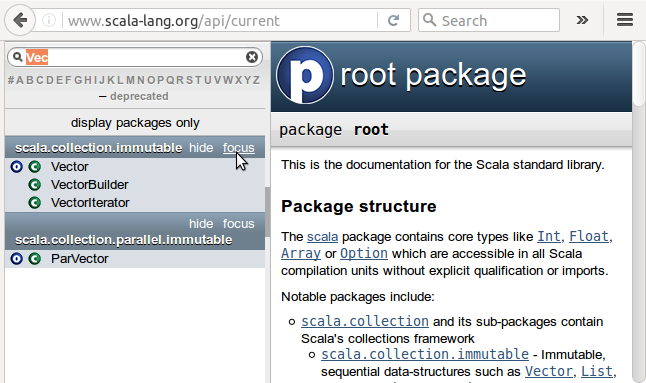
\includegraphics[width=0.8\textwidth]{../img/scaladoc/scaladoc-root}

     \caption{ \scaladoc.}
    \label{fig:scaladoc:root-package}
\end{figure}

Om du är speciellt intresserad av, t.ex., paketet \code{scala.collection.immutable}, kan du klicka \textbf{focus} för att begränsas visningen till att endast innehålla typerna i detta paket.

Om du söker efter typen där en viss metod är implementerad, men inte vet riktigt i vilken klass den finns, kan du klicka på bokstaven som metodnamnet börjar på i listan med bokstäver under den övre vänstra sökrutan. Då får du en lista med allt möjligt som börjar på F, så som visas i figur \ref{fig:scaladoc:find}. Sök i listan med din webbläsares sökfunktion (Ctrl+F) efter ''fill'', så hittar du alla typer som implementerar metoden \code{fill}. 

\begin{figure}[H]
\centering
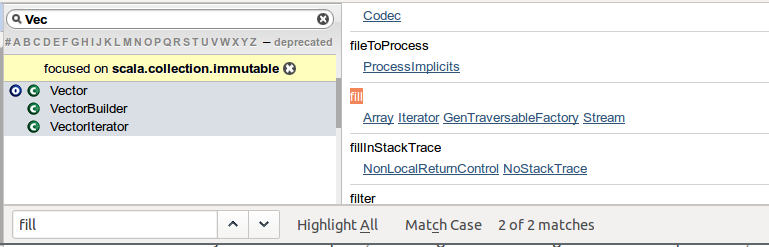
\includegraphics[width=1.0\textwidth]{../img/scaladoc/scaladoc-find-fill}

     \caption{ \scaladoc.}
    \label{fig:scaladoc:find}
\end{figure}

Om du klickar vidare, i detta exempel på länken till klassen Array, kan du sedan klicka på länken till källkoden i \texttt{array.scala} för att se implementationen på GitHub; sök på sidan med din webbläsares sökfunktion Ctrl+F efter ''def fill''.





Om du klickar på den typ du är intresserad av, t.ex. klassen Vector, får du upp en sida med en mängd information, inklusive alla metoder, även ärvda. Figur \ref{fig:scaladoc:vector} visar hur en sökning bland alla metoder i Vector initieras i sökrutan nere till höger, vilken kommer att visa metoder som börjar på ''rev'', här skrollas fönstret till metoden \code{reverse} längre ner på sidan.

Genom att klicka på det den gröna cirkeln med bokstaven C överst i dokumentationsfönstret, växlar du till vyn för kompanjonsobjektet där du hittar alla fabriksmetoder för Vector, även ärvda, t.ex. \code{fill} som du kan söka efter i sökrutan. 



\begin{figure}[H]
\centering
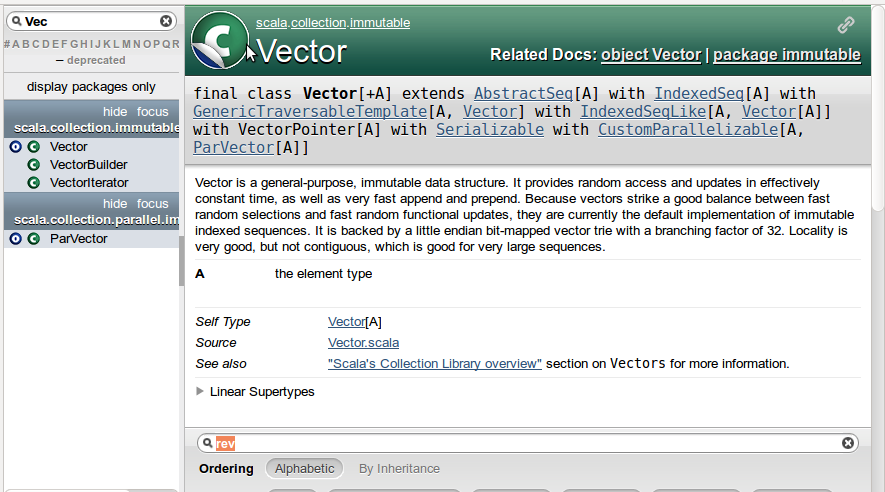
\includegraphics[width=1.0\textwidth]{../img/scaladoc/scaladoc-vec}

     \caption{ \scaladoc.}
    \label{fig:scaladoc:vector}
\end{figure}


\subsection{Skriva dokumentationskommentarer för scaladoc}


Verktyget \scaladoc~läser kommentarer som börjar med \verb|/**| och slutar med \verb|*/| och associeras till efterföljande deklaration. Notera de dubbla asteriskerna. Alla rader som följer efter \verb|/**| ska, enligt konventionen för Scalas dokumentationskommentarer, börja med en asterisk \code|*| med indrag med flera blanksteg så att den hamnar under \textit{andra} asterisken i öppningskommentaren, som nedan:
\begin{Code}
/** Först kommer en sammanfattning på en enda rad. 
  * 
  * Sedan kommer eventuellt en mer detaljerad beskrivning, 
  * som kan vara flera rader lång.
  */
\end{Code}
Dokumentationskommentaren slutar med \code|*/| rakt under asterisk-kolumnen.

I figur \ref{fig:scaladoc:mio} på sidan \pageref{fig:scaladoc:mio} visas exempel på dokumentationskommentarer. Annoteringen \verb|@param| i början på en rad ger en speciell kommentar angående parametrar. Annoteringen \verb|@return| i början av en rad ger en speciell kommentar angående vad som returneras vid metodanrop.


\subsection{Generera dokumentation med scaladoc}


Du genererar en dokumentationssajt med terminalkommandot \scaladoc~följt av en eller flera källkodsfiler. Med optionen \code{-d} anger du i vilket bibliotek sajten ska sparas. Du visar sajten genom att öppna filen \code{index.html} i en webbläsare. Nedan visas hur dokumentationen genereras för källkodsfilen i figur \ref{fig:scaladoc:mio}.
\begin{REPLnonum}
$ scaladoc mio.scala -d apidoc
$ firefox apidoc/index.html
\end{REPLnonum}

I figur \ref{fig:scaladoc:webpage} på sidan \pageref{fig:scaladoc:webpage} visas delar av en webbsida som genererats utifrån koden i figur \ref{fig:scaladoc:mio} på sidan \pageref{fig:scaladoc:mio}. För de publika metoder där ingen dokumentationskommentar finns, visas ändå metodens signatur med parametrar, parametertyper, och returtyp. Medlemmar som deklareras \code{private} visas inte, men om man klickar på knappen \Button{All} bredvid rubriken \textbf{Visibility} visas medlemmar som är deklarerade \code {protected}.

Om du klickar på symbolen \Forward~till vänster om metodsignaturen, ändras den till symbolen \MoveDown  ~som indikerar att den mer detaljerade beskrivningen av parametrar etc. har vecklats ut (i den mån detaljerade kommentarer finns). 

Om du vill ha övergripande dokumentation om ett paket \code{x}, ges det speciella objektet \code{package object x} en dokumentationskommentar med sådan information. Ofta innehåller \code{package object} medlemmar som man vill ska bli synliga vid import av paketet, så som variabler, metoder och implicita medlemmar som inte har någon annan naturlig hemvist.

\begin{figure}[b]
\scalainputlisting[numbers=left, basicstyle=\ttfamily\fontsize{9}{11}\selectfont]{../util/mio.scala}
    \caption{Dokumentationskommentarer som kan läsas av \scaladoc för att generera en dokumentations-webbsajt. Sådana kommentarer börjar  med snedstreck och dubbla asterisker, se bl.a. raderna 8--13 ovan.}
    \label{fig:scaladoc:mio}
\end{figure}

\begin{figure}[t]
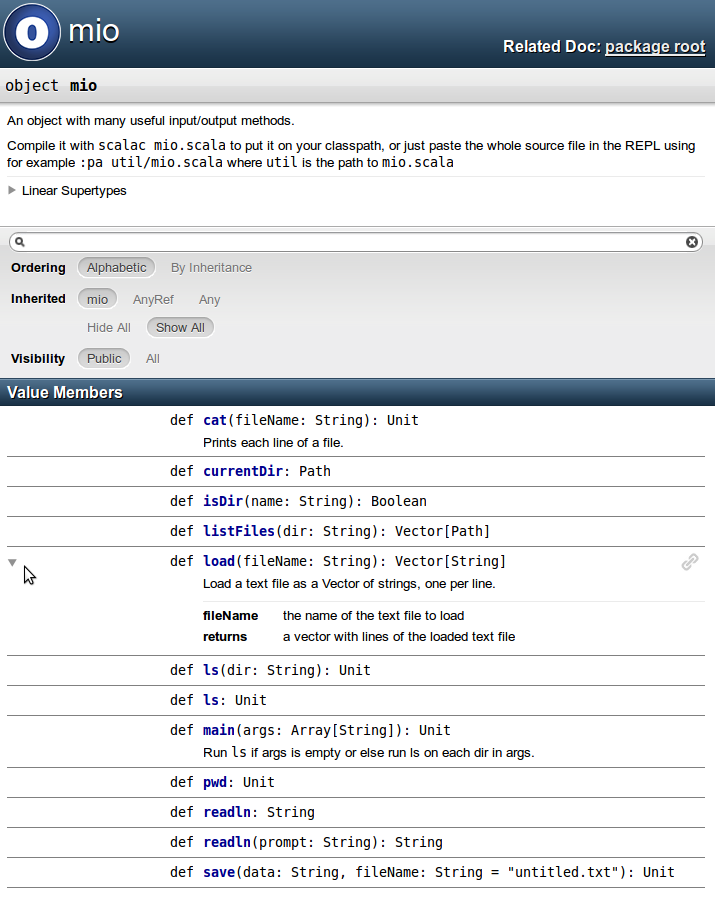
\includegraphics[width=1.0\textwidth]{../img/scaladoc/scaladoc-mio}
    \caption{Delar av en webbsida genererad med hjälp av \scaladoc. Mer detaljerade beskrivningar kan i förekommande fall vecklas ut eller in om man växlar mellan \Forward~och \MoveDown.}
    \label{fig:scaladoc:webpage}
\end{figure}


\subsection{Lära mer om scaladoc}

\begin{itemize}[leftmargin=*]

\item En video med tips om hur du söker och navigerar i \scaladoc-dokumentation: 
\\
\url{http://docs.scala-lang.org/overviews/scaladoc/interface.html}

\item
Riktlinjer för hur du skriver dokumentationskommentarer: \\
\url{http://docs.scala-lang.org/style/scaladoc.html}

\item Länksida till mer detaljerade beskrivningar: \\
\url{https://wiki.scala-lang.org/display/SW/Writing+Documentation} \\
inkluderande bland annat:

\begin{itemize}[nolistsep]
\item En beskrivning av syntaxen för formatering: \\
\url{https://wiki.scala-lang.org/display/SW/Syntax} 

\item En beskrivning av speciella annoteringar, t.ex. \code{@param}: \\
\url{https://wiki.scala-lang.org/display/SW/Tags+and+Annotations} 

\end{itemize}

\item Kör kommandot \texttt{ scaladoc -help } för att se användbara optioner.

\item \texttt{sbt doc} är ett smidigt sätt att generera api-dokumentation. Läs mer om \texttt{sbt} och api-dokumentation här: \\
\url{http://www.scala-sbt.org/0.13/docs/Howto-Scaladoc.html}


\end{itemize}

\clearpage

\section{javadoc}
\newcommand{\javadoc}{\texttt{javadoc}}


Med Java JDK följer dokumentationsverktyget \javadoc, som utifrån dokumentationskommentarer i Java-kod genererar en webbsajt med navigationslänkar. Webbsidor genererade med \javadoc~erbjuder inte samma funktioner för sökning och filtrering som \scaladoc, men det fungerar bra hitta det man söker om navigationslänkarna används tillsammans med webbläsarens inbyggda sökfunktion (Ctrlf+F).

\subsection{Använda dokumentation genererad med javadoc}

I figur \ref{fig:javadoc:overview} visas exempel på \javadoc~för biblioteket \code{cslib}. Om du klickar på ett paket kan du navigera till en översikt av innehållet i paketet. Om du klickar på en klass får du en översikt av klassens medlemmar, så som visas i \ref{fig:javadoc:class}.  Om du t.ex. klickar på ett metodnamn får du se mer detaljerade kommentarer. 

Ramarna till vänster på webbsidorna innehåller länkar till paket och klasser. Om du klickar på länken \textit{All Classes} överst till vänster för du en lista med navigationslänkar till alla tillgängliga klasser.De gulmarkerade rubrikerna visar vilken vy som är aktiv och navigationslänkar skrivs med blå text.

\begin{figure}
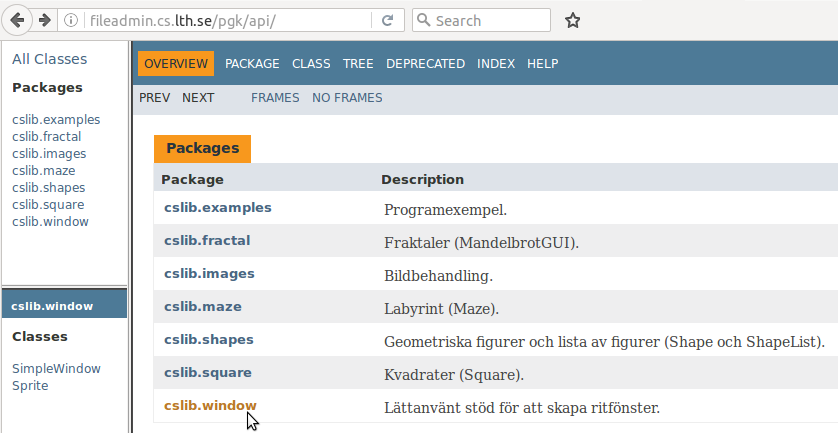
\includegraphics[width=1.0\textwidth]{../img/javadoc/javadoc-overview}
    \caption{Delar av en webbsida genererad med hjälp av \javadoc.}
    \label{fig:javadoc:overview}
\end{figure}



\begin{figure}
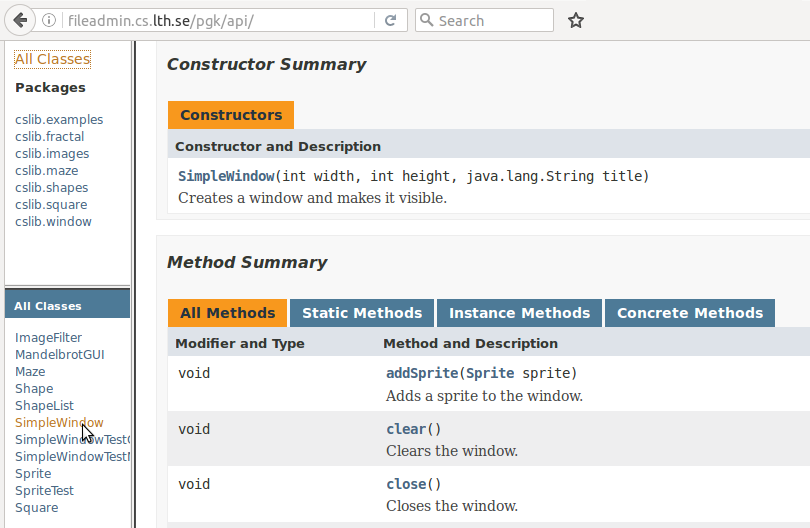
\includegraphics[width=1.0\textwidth]{../img/javadoc/javadoc-class}
    \caption{Delar av en webbsida med klassdokumentation genererad med hjälp av \javadoc.}
    \label{fig:javadoc:class}
\end{figure}






\subsection{Skriva dokumentationskommentarer för javadoc}

Kommentarer för \javadoc~och \scaladoc~ser ganska lika ut, även om det finns några skillnader. Det finns t.ex. inte lika många styrtecken för layouten i \javadoc~som i \scaladoc, och konventionen i Java är fyra blankstegs indrag och att fortsättningsrader i dokumentationskommentarer börjar asterisken under \textit{första} asterisken i öppningskommentaren. 

Nedan visas delar av \javadoc-kommentarerna för klassen \code{SimpleWindow} och dess konstruktor:
\begin{Code}[language=Java]
package cslib.window;
 
/** A simple window to draw in */
public class SimpleWindow {
   /**
    * Creates a window and makes it visible.
    * 
    * @param width   the width of the window
    * @param height  the height of the window
    * @param title   the title of the window
    */
    public SimpleWindow(int width, int height, String title) {
        ...
\end{Code}
Annoteringen \verb|@param| i början på en rad ger en speciell kommentar angående en parameter. Vid dokumentation av metoder kan annoteringen \verb|@return| användas i början av en rad för att skapa en speciell kommentar angående vad som returneras.

Övergripande dokumentation om innehållet i ett paket läggs i en textfil i paketets katalog med namnet \texttt{package-info.java}, se till exempel här: \\ {\href{https://github.com/lunduniversity/introprog/tree/master/workspace/cslib/src/main/java/cslib/window}{\small github.com/lunduniversity/introprog/tree/master/workspace/cslib/src/main/java/cslib/window}


Du kan läsa mer om hur man skriver \code{javadoc}-kommentarer här:\\
\href{http://www.oracle.com/technetwork/java/javase/documentation/index-137868.html}{www.oracle.com/technetwork/java/javase/documentation/index-137868.html}

% conversation of diffs between javadoc and scaladoc:
%  https://groups.google.com/forum/#!msg/scala-user/q-Vw03zcIVs/CaTR5XL-BQAJ

\subsection{Generera dokumentationskommentarer för javadoc}

Om du står i den katalog där din källkod finns, kan du med nedan kommando i terminalen gå igenom alla paket och underpaket och generera \javadoc-webbsidor i katalogen \texttt{doc}. Du kan därefter öppna dokumentationen i en webbläsare.
\begin{REPLnonum}[basicstyle=\color{white}\ttfamily\fontsize{9}{11}\selectfont]
$ javadoc -d doc -encoding UTF-8 -charset UTF-8 -sourcepath . -subpackages . *
$ firefox doc/index.html
\end{REPLnonum}
Ett smidigt sätt att generera både \scaladoc~och \javadoc~ är att använda \texttt{sbt}; det är bara att skriva \code{ sbt doc } i terminalen så genereras alla dokumentation för både Scala och Java i den katalog som \texttt{sbt} meddelar i sin resultatutskrift.

Om du lägger in nedan i \code{settings} i din \code{build.sbt} fungerar även svenska bokstäver och andra specialtecken på alla plattformar.
\begin{Code}
  javacOptions in (Compile, doc) ++= Seq(
    "-encoding", "UTF-8", 
    "-charset", "UTF-8", 
    "-docencoding", "UTF-8")
\end{Code}  

\noindent Du kan också använda din IDE för att köra \javadoc. I Eclipse, använd menyn \MenuArrow{Project}\Menu{Generate Javadoc...}, medan du i IntelliJ hittar motsvarande i menyn \MenuArrow{Tools}\Menu{Generate Javadoc...}
%!TEX encoding = UTF-8 Unicode
%!TEX root = ../compendium.tex

\chapter{Integrerad utvecklingsmiljö}\label{appendix:ide}

\section{Vad är en integrerad utvecklingsmiljö?}

En integrerad utvecklingsmiljö \Eng{integrated development environment, IDE} samlar ett flertal verktyg, inklusive en avancerad \textbf{editor} (se appendix \ref{appendix:edit}), för att skapa, köra och testa program. Det finns flera utvecklingsmiljöer att välja mellan, som kan användas för både Scala och Java.

En IDE ger stöd för auto-komplettering \Eng{auto completion} där tillgängliga metoder visas i en lista och resten av ett namn kan fyllas efter att du skrivit de första bokstäverna i namnet. En IDE kan hjälpa dig med formattering och även skapa skelettkod utifrån \textbf{kodmallar} \Eng{code templates}. Med \textbf{felindikering} \Eng{error highlighting} får du understrykning av vissa fel direkt i koden och ibland kan du även få hjälp med förslag på åtgärder för att rätta till enkla fel. Funktioner för \textbf{avlusning} \Eng{debugging} hjälper dig att felsöka medan du kör din kod. Med funktioner för \textbf{omstrukturering} \Eng{refactoring} av kod får du hjälp av editorn i samarbete med kompilatorn att göra omfattande strukturförändringar i många kodfiler samtidigt, t.ex. namnbyten med hänsyn taget till synlighetsregler.  

Alla dessa avancerade funktioner kan öka produktiviteten avsevärt, men samtidigt tar de tid att lära sig och en IDE kan kräva mycket datorkraft och viss väntetid jämfört med en vanlig, fristående editor. I början kan all funktionalitet upplevas som överväldigande och det kan vara svårt att hitta i alla menyer och inställningar. Ska man bara skriva ett litet, enkelt program, eller göra några mindre ändringar, är det många som föredrar en fristående, snabbstartad kodeditor före en fullfjädrad, tungrodd IDE. Å andra sidan kan en IDE hjälpa till att upptäcka vad som finns i ett api och autokompletteringsfunktionen hjälpa stort när man upptäcker och experimenterar med en okänd kodmassa.


\section{Kojo}\label{appendix:kojo}

\subsection{Installera Kojo}

\href{http://www.kogics.net/kojo-download}{www.kogics.net/kojo-download}

\subsection{Använda Kojo}

\begin{table}[h]
\caption{Några av sköldpaddans funktioner. Se även \href{http://lth.se/programmera}{lth.se/programmera}}
\vspace{1em}\small
\begin{tabular}{lll}
\emph{Svenska} & \emph{Engelska} & \emph{Vad händer?}\\ \hline
\tt fram     & \tt forward     & Paddan går 25 steg frammåt.           \\
\tt fram(50) & \tt forward(50) & Paddan går 50 steg frammåt.           \\
\tt höger    & \tt right       & Paddan vrider sig 90 grader åt höger. \\
\code+upprepa(10){???}+ & \code+repeat(10){???}+  & Repetition av ??? 10 gånger. \\
\end{tabular}
\end{table}

\noindent Koden för den svenska paddans api finns här:
\href{https://bitbucket.org/lalit\_pant/kojo/src/tip/src/main/scala/net/kogics/kojo/lite/i18n/svInit.scala?at=default\&fileviewer=file-view-default\#svInit.scala-26}{bitbucket.org/lalit\_pant/kojo/}

\section{Eclipse och ScalaIDE}\label{appendix:ide:eclipse}

\subsection{Installera Eclipse och ScalaIDE}\label{appendix:ide:eclipse:install}

\subsection{Använda Eclipse och ScalaIDE}\label{appendix:ide:eclipse:use}

\subsubsection{Ladda ner och importera projekt från kursens workspace}

TODO: skriv mer här

\begin{itemize}
\item Ladda ner kursens workspace här: \url{http://cs.lth.se/pgk/workspace}
\item Packa upp filen på lämpligt ställe.
\item Starta Eclipse med ScalaIDE-plugin (för installation se \ref{appendix:ide:eclipse:install}).
\item Bläddra till biblioteket du nyss packade upp, ungefär som i \ref{fig:eclipse:ide:open}
\begin{figure}[H]
\centering
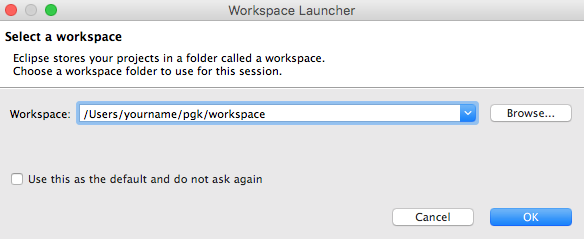
\includegraphics[width=0.7\textwidth]{../img/pirates/selectws.png}
\caption { \emph{Öppna workspace:} Bläddra fram till kursens workspace och klicka {\bf OK. }}
\label{fig:eclipse:ide:open}
\end{figure}

\item Gå vidare från startskärmen genom att välja {\bf Workspace}, se Fig.\ref{fig:eclipse:ide:selectws}.
\begin{figure}[H]
\centering
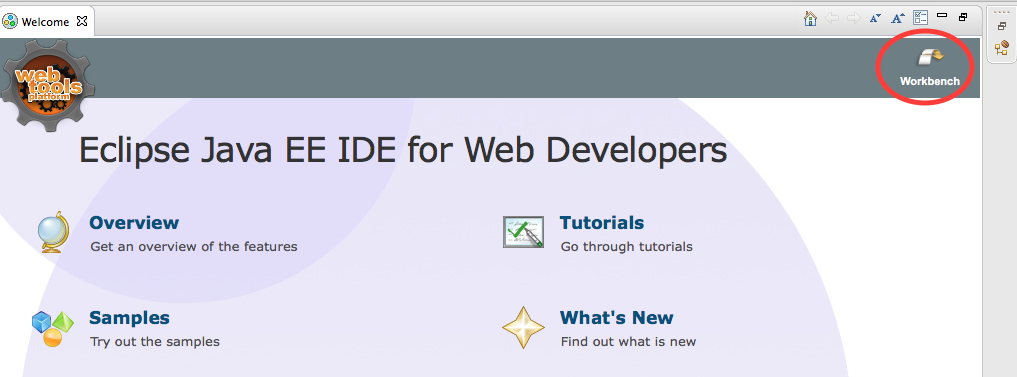
\includegraphics[width=0.7\textwidth]{../img/pirates/selectws2.png} \\

\caption {Välj {\bf workspace}.}
\label{fig:eclipse:ide:selectws}
\end{figure}

\item Uppe till höger ser du vilken \emph{vy} du har. I Eclipse kommer vi växla mellan Scala, Java och debug-vyer. Dessa läggs till via listan som nås genom den fönsterliknande ikonen enligt Fig.~\ref{fig:eclipse:ide:changeview}. Du ska ha {\bf Scala} igång.

\begin{figure}[H]
\centering
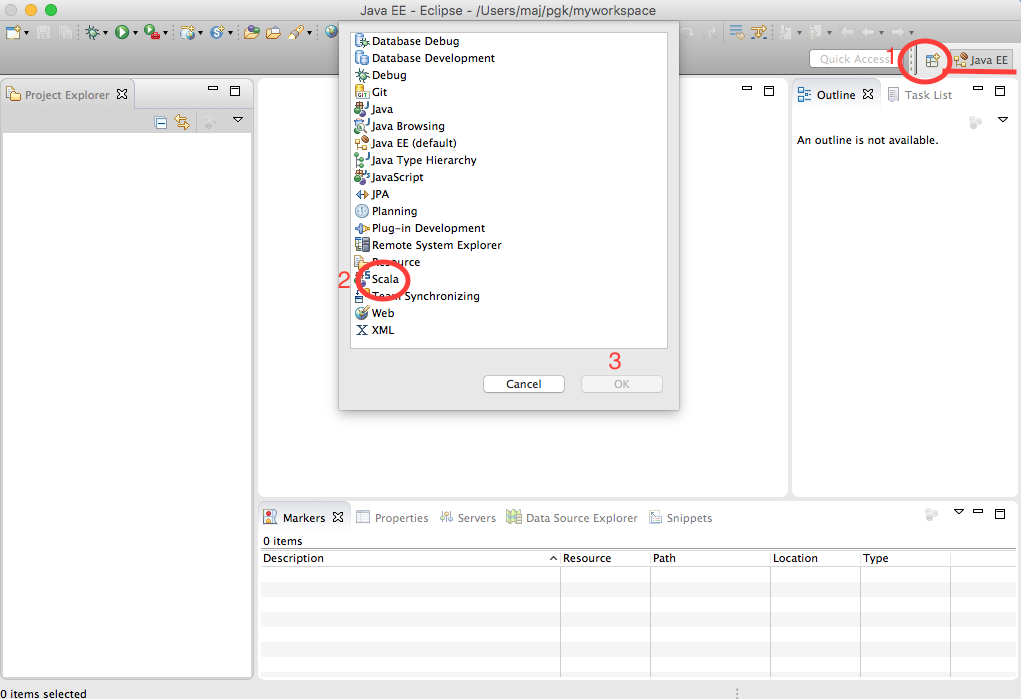
\includegraphics[width=0.7\textwidth]{../img/pirates/selectscala.png} 

\caption {Lägg till vyer från listan med installerade plugin.}
\label{fig:eclipse:ide:changeview}
\end{figure}

\item Högerklicka i {\bf Project Explorer} och välj {\bf New} -> {\bf Scala Project}, se Fig.~\ref{fig:eclipse:ide:createproject}. Importera existerande project genom att genom att avmarkera \emph{Use default location} och bläddra till katalogen för respektive laboration och sen {\bf Finish}, se exempel i Fig.~\ref{fig:eclipse:ide:import} (namnet sätts automatiskt). Du kan också skapa nya projekt genom att ange ett projektnamn direkt och sen klicka {\bf Finish} enligt Fig.~\ref{fig:eclipse:ide:newproject}.

\begin{figure}[H]
\centering
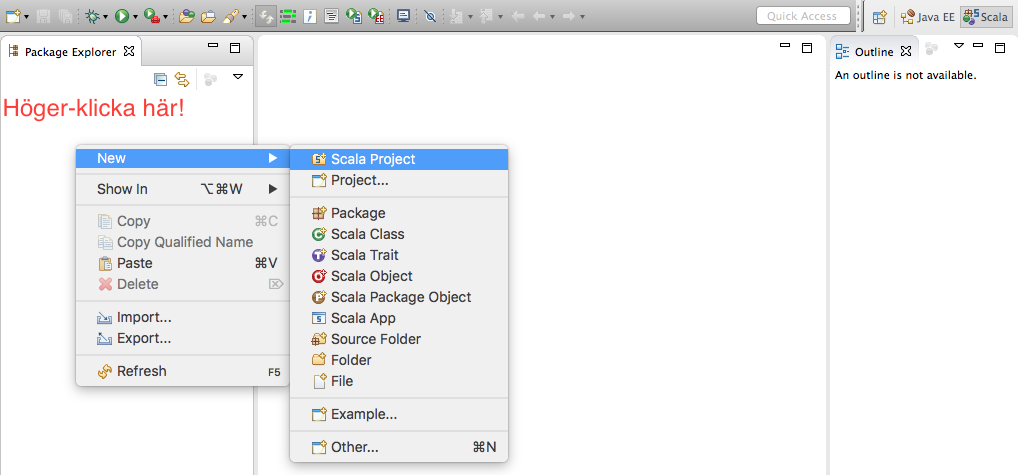
\includegraphics[width=0.7\textwidth]{../img/pirates/createproject.png} 

\caption {Välj att {\bf Scala Project} i menyerna.}
\label{fig:eclipse:ide:createproject}
\end{figure}
\begin{figure}[H]
\centering
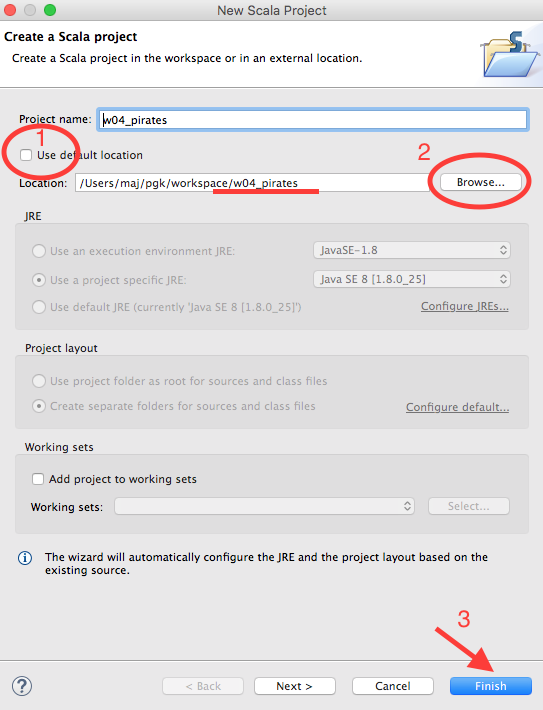
\includegraphics[width=0.5\textwidth]{../img/pirates/importproject.png} 

\caption {Importera existerande projekt genom att ange sökvägen.}
\label{fig:eclipse:ide:import}
\end{figure}

\begin{figure}[H]
\centering
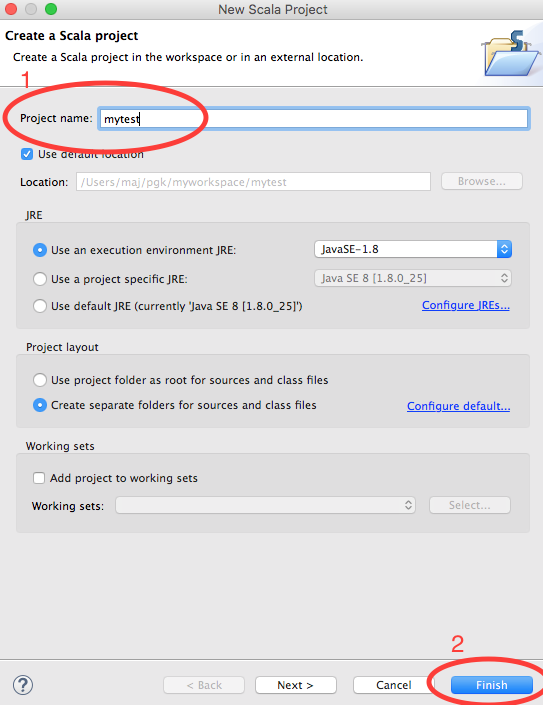
\includegraphics[width=0.5\textwidth]{../img/pirates/nameproject.png} 

\caption {Skapa ett nytt projekt genom att ange namn.}
\label{fig:eclipse:ide:newproject}
\end{figure}


\item Du skapar nya klasser och objekt på liknande sätt, genom att högerklicka och välja {\bf New}, se exempel i Fig.~\ref{fig:eclipse:ide:createobject}


\begin{figure}[H]
\centering
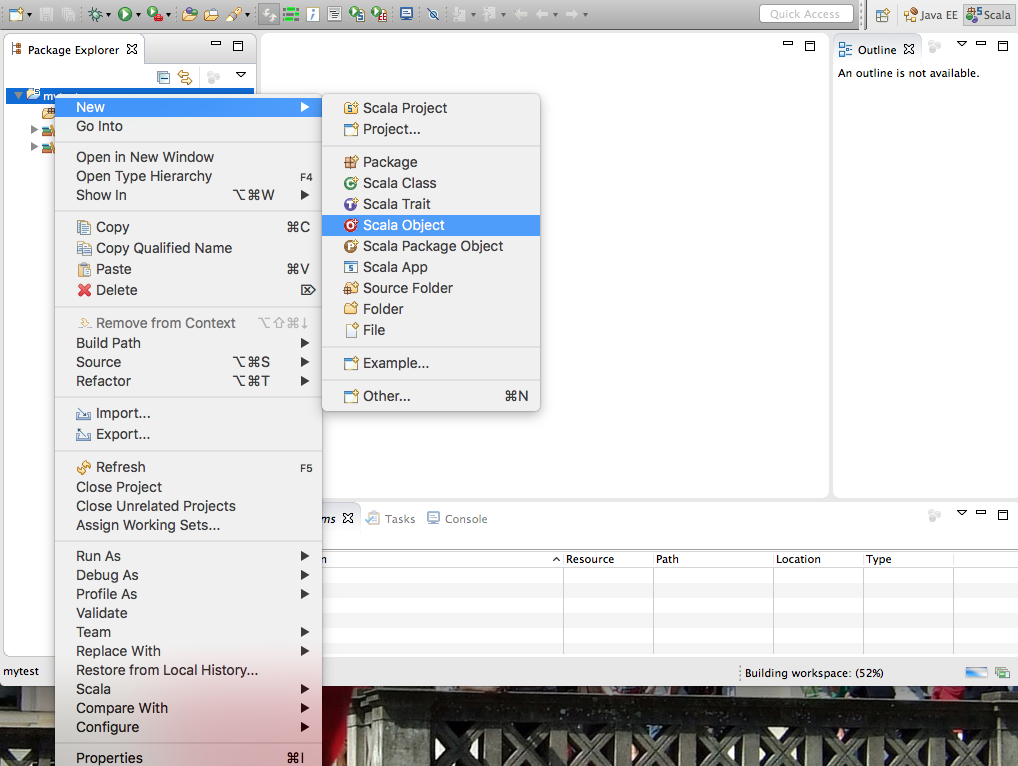
\includegraphics[width=0.7\textwidth]{../img/pirates/createobject.png} 
\caption {Skapa ett nytt objekt via menyerna.}
\label{fig:eclipse:ide:createobject}
\end{figure}

\item Skriv ett main-program och exekvera det genom att markera klassen i {\bf Project Explorer} och sen klicka på den gröna pilen. Utskrifter kommer till konsolen längst ner. 

\begin{figure}[H]
\centering
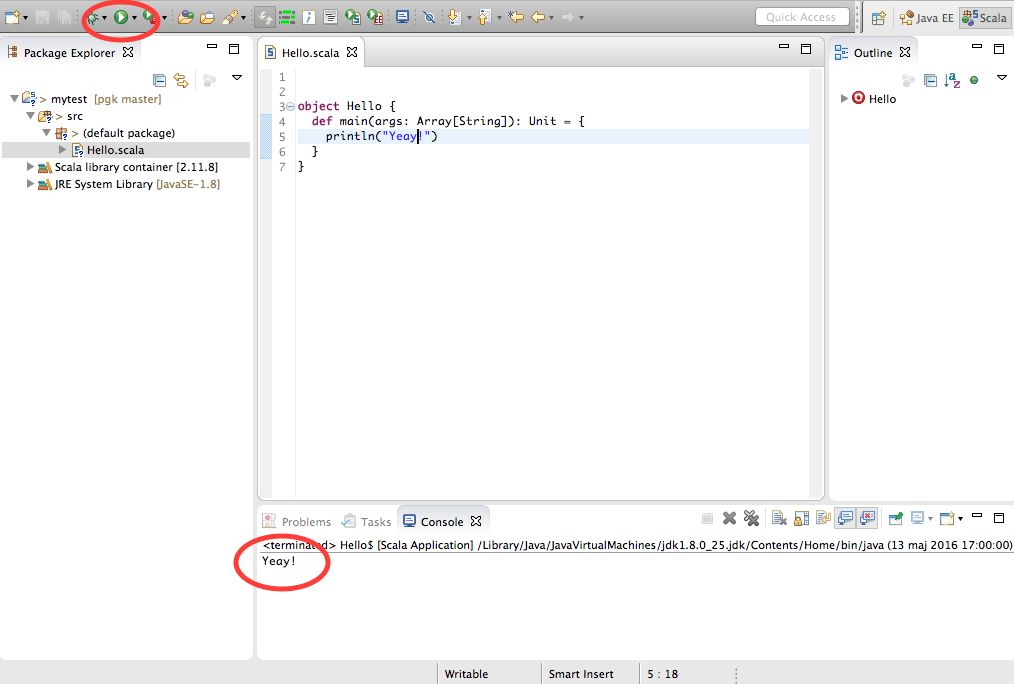
\includegraphics[width=0.7\textwidth]{../img/pirates/exekvera.png} 
\caption {Exekvera med den gröna pilen.}
\label{fig:eclipse:ide:exec}
\end{figure}
\end{itemize}




%!TEX encoding = UTF-8 Unicode
%!TEX root = ../compendium.tex

\chapter{Byggverktyg}

\section{Vad gör ett byggverktyg?}

\section{Byggverktyget sbt}

\subsection{Installera sbt}

\subsection{Använda sbt}
%!TEX encoding = UTF-8 Unicode
%!TEX root = ../compendium.tex


\chapter{Versionshantering och kodlagring}

\section{Vad är versionshantering?}

\textbf{Versionshantering}\footnote{\href{https://en.wikipedia.org/wiki/Version_control}{en.wikipedia.org/wiki/Version\_control}} \Eng{version control eller revision control} av mjukvara innebär att hålla koll på olika versioner av koden i ett utvecklingsprojekt allteftersom koden ändras. Versionshantering är en deldisciplin inom \textbf{konfigurationshantering} \Eng{software configuration managament} som inbegriper allt i processen för att identifiera, besluta, genomföra och följa upp ändringar.

En viktig del av versionshantering är att \textit{lagra} olika versioner av koden allt eftersom den utvecklas, så att tidigare versioner kan \textit{återskapas} vid behov. Ett bra verktygsstöd och en väldefinierad arbetsprocess för versionshanteringen, som alla i utvecklingsprojektet följer, möjliggör att flera utvecklare kan \textit{arbeta parallellt} med att sammanfoga \Eng{merge} varandras tillägg och ändringar i den gemensamma kodbasen utan att det blir kaos och förvirring.

God versionshantering är helt avgörande för utvecklarnas produktivitet, speciellt för stora projekt med många utvecklare som jobbar parallellt mot en omfattande kodbas med många olika interna och externa komponenter. 
Men även ett litet projekt med en enda utvecklare kan ha god nytta av ett versionshanteringsverktyg och ett disciplinerat förfarande för att namge versioner, t.ex. för att kunna återskapa tidigare versioner av projektets olika kodfiler när en ändring visar sig mindre lyckad.   

Det finns flera olika modeller för hur kodlagringen sker:
\begin{itemize}
\item \textbf{lokal}; alla utvecklare jobbar i samma, lokala filsystem där alla olika versioner lagras.
\item \textbf{centraliserad}; ett repositorium (förk. repo), alltså en databas med koden, finns centralt på en server som alla jobbar mot med hjällp av en versionshanteringsklient.
\item \textbf{distribuerad}; alla utvecklare har sitt eget lokala repo och varje utvecklare initierar enskilt delning av ändringar mellan olika repo. 
\end{itemize}


\section{Versionshanteringsverktyget Git}

Det finns många olika versionshanteringsverktyg\footnote{\href{https://en.wikipedia.org/wiki/List_of_version_control_software}{https://en.wikipedia.org/wiki/List\_of\_version\_control\_software}}
 som använder olika modeller för kodlagring; lokal, centraliserad, distribuerad eller kombinationer därav. 
På senare tid har verktyget \textbf{Git}\footnote{\href{https://en.wikipedia.org/wiki/Git_(software)}{https://en.wikipedia.org/wiki/Git\_(software)}} fått en stark ställning, speciellt i öppenkällkodsvärlden. Git utvecklades ursprungligen av Linus Torvalds för att versionshantera Linuxkärnan, men har växt till ett omfattande öppenkällkodsprojekt med stor spridning och många användare och bidragsgivare. 

Git är skapad för \textbf{distribuerad} versionshantering där var och en kan jobba snabbt och smidigt i sitt eget lokala repo, utan att behöva vänta på att en klient ska synkronisera koden med ett centralt repo på en server över nätverket. Ändringar delas mellan repo på begäran ev enskilda utvecklare. 

Varje ny version av koden lagras som en avgränsad mängd ändringar sedan förra versionen, en s.k. \textbf{commit}%
\footnote{På svenska kan t.ex. ''inlämning'' användas, men låneordet commit är redan etablerat.}%
, och hanteras internt av Git i en lokal databas i katalogen \code{.git} som ligger överst i din projektkatalog. Genom olika kommandon i terminalen, eller via en klient med ett grafiskt användargränssnitt, kan din kod överföras till och från den lokala koddatabasen, alternativt delas med andra repon via nätet. 

Det finns en välskriven bok kallad \textit{''Pro Git''} som förklarar Git på djupet och är tillgänglig fritt här: 
\url{https://git-scm.com/book/en/v2}.
Läs kapitel 1 och 2 så får du en bra grund att stå på. 

Dessa termer är bra att kunna utantill innan du kör igång med Git:
\newcommand{\TermItem}[3]{\item \textbf{#1} (\textit{substantiv}: #2, \textit{verb}: #3).}
\begin{itemize}

\item \textbf{repo} (\textit{substantiv}: ett repositorium, \textit{eng. a repository}) En koddatabas med ändringshistorik. 

\TermItem{commit}{en inlämning}{att lämna in} 
  En avgränsad mängd nya ändringar lämnas in i det lokala repot. Repots ändringshistorik utgörs av sekvensen av alla inlämningar.

\TermItem{push}{en leverans}{att leverera, att trycka upp} En eller flera inlämningar trycks upp till ett annat repo.

\TermItem{pull}{en hämtning}{att hämta, att dra ner} En eller flera inlämningar dras ner från ett annat repo.

\TermItem{merge}{en ihopslagning}{att sammanfoga} En eller flera inlämningar slås samman till en ny inlämning. 

\item \textbf{merge conflict} (\textit{substantiv}: en sammanfogningskonflikt, \textit{eng. a merge conflict}) Problem vid sammanfogning; ändringar kan inte enkelt sammanfogas på ett entydigt sätt.

\item \textbf{pull request} (förk. PR, \textit{substantiv}: en hämtningsbegäran, \textit{verb}: att begära en hämtning). Utvecklare A ber en annan utvecklare B att hämta en eller flera inlämningar från A:s repo och sammanfoga med B:s repo.

\end{itemize}

\subsection{Installera git}

Git finns förinstallerat på LTH:s Linuxdatorer. Du kan kolla om Git redan finns på din maskin genom att skriva \code{git help} i terminalen. 

Det finns bra instruktioner om hur du installerar Git på din egen maskin här: \url{https://git-scm.com/book/en/v2/Getting-Started-Installing-Git}

Om du vill ha en Git-klient med grafiskt användargränssnitt finns det många att välja på, se här:  \url{https://git-scm.com/downloads/guis} 

Om du inte vet vilken du ska välja, prova GitKraken som är öppen, fri och gratis och finns för alla plattformar och kan laddas ner här: \\ \url{https://www.gitkraken.com/}


\subsection{Anpassa Git}

Innan du börjar använda git, konfigurera ditt användarnamn och din email med nedan terminalkommando, där du anger ditt användarnamn i stället för \code{fornamnefternamn} och din mejladress i stället för \code{mejladr@plats.se}:
\begin{REPLnonum}
$ git config --global user.name fornamnefternamn
$ git config --global user.email mejladr@plats.se
\end{REPLnonum}
Det är bra att välja \textit{ett} användarnamn, för \textit{alla} repo, även kodlagringsplatser på nätet; förslagsvis \code{fornamnefternamn} utan svenska tecken,  så att du blir lätt att känna igen, speciellt om du jobbar med öppen källkod där ditt namn kommer associerat med alla de kodbidrag du gör under ditt yrkesliv.

Läs mer om hur du gör andra inställningar här, t.ex. hur du anger vilken editor som git startar när du ska skriva commit-beskrivningar: \\ \url{https://git-scm.com/book/en/v2/Getting-Started-First-Time-Git-Setup}
  
  
\subsection{Använda git}

Nedan listas några vanliga terminalkommandon i Git.

\begin{itemize}[leftmargin=*]

\item Skapa ett repo i en katalog:
\begin{REPLnonum}
$ cd myproject
$ git init
\end{REPLnonum} 

\item Se vilka filer som ändrats och ännu ej lämnats in:
\begin{REPLnonum}
$ git status
$ git status -s
\end{REPLnonum} 

\item Se vilka ändringar som gjorts i filer som ännu ej lämnats in:
\begin{REPLnonum}
$ git diff 
\end{REPLnonum} 

\item Se vilka inlämningar som finns i ändringshistoriken:
\begin{REPLnonum}
$ git log 
$ git log --oneline -5
\end{REPLnonum} 

\item Lägga till filer som ska ingå i nästa inlämning och sedan göra inlämningen och ge den en bra beskrivning som förklarar vad inlämningen omfattar:
\begin{REPLnonum}
$ git add *.scala
$ git commit -m 'initial project version'
\end{REPLnonum} 

\item Ångra alla tillägg inför inlämning (ändringarna finns kvar och kan läggas till igen om du vill):
\begin{REPLnonum}
$ git reset 
\end{REPLnonum} 

\item Skippa alla ej tillagda ändringar i filen \code{filename}.
\\VARNING! Senaste ändringar förloras för alltid.  
\begin{REPLnonum}
$ git checkout filename 
\end{REPLnonum} 

\end{itemize}
 
\TODO Förhindra versionshantering av vissa filer .gitignore
 
  
\section{Kodlagringsplatser på nätet}

\begin{itemize}

\TermItem{fork}{en förgrening av ett helt repo}{att förgrena ett repo, ''forka''} Genom att forka ett repo får du en kopia som du kan utveckla separat; det blir då möjligt för dig att lämna in ändringar (''commita''), även om du inte har rättigheter att leverera (''pusha'') till originalet. Gör en ändringsbegäran (Pull Request, PR) om du vill bidra med dina ändringar, så kan ägaren av orginalet sedan välja att sammanfoga (''merga'') dina ändringar med orginalet.

\item \textbf{upstream} (\textit{preposition}: uppströms, \textit{substantiv}: uppströmsrepo) Ett uppströmsrepo utgör orginal till ett förgrenat repo (en ''fork''). 
\begin{itemize}

\item Här beskrivs hur du länkar en förgrening uppströms: \\ 
{\small\url{https://help.github.com/articles/configuring-a-remote-for-a-fork/}}

\item Här beskrivs hur du synkar en förgrening uppströms:\\
{\small\url{https://help.github.com/articles/syncing-a-fork/}}

\end{itemize}

\end{itemize}

Några användbara kommandon:

\begin{itemize}
\item Skapa en lokal kopia av ett fjärran \Eng{remote} repo på kodlagringsplatsen GitHub:
\begin{REPLnonum}
$ git clone --depth 1 https://github.com/lunduniversity/introprog
\end{REPLnonum} 

\item Dra ner nya inlämningar från ett fjärran repo:
\begin{REPLnonum}
$ git pull 
\end{REPLnonum} 

\item Trycka upp nya lokala inlämning till ett fjärran repo:
\begin{REPLnonum}
$ git push 
\end{REPLnonum} 

\end{itemize}




\subsection{GitLab}


\subsection{GitHub}

\subsubsection{Installera klienten för GitHub}

\subsubsection{Använda GitHub}


\subsection{BitBucket}

\subsubsection{Installera SourceTree}

\subsubsection{Använda BitBucket och SourceTree}

%!TEX encoding = UTF-8 Unicode
%!TEX root = ../compendium.tex

\chapter{Virtuell maskin}\label{appendix:vbox}

\section{Vad är en virtuell maskin?}

Du kan köra alla kursens verktyg i en så kallad virtuell maskin (vm). Det är ett enkelt och säkert sätt att installera ett nytt operativsystem i en ''sandlåda'' som inte påverkar din dators ursprungliga operativsystem. 

\section{Installera kursens vm}
Det finns en virtuell maskin förberedd med alla verktyg som du behöver förinstallerade. Gör så här:
\begin{enumerate}
\item     Installera VirtualBox v5 här: \\ \url{https://www.virtualbox.org/wiki/Downloads}
\item     Ladda ner filen vbox.zip här: \\ \url{http://fileadmin.cs.lth.se/pgk/vbox.zip} \\ OBS! Då filen är på nästan 4GB kan nedladdningen ta mycket lång tid.
\item     Packa upp filen vbox.zip i biblioteket ''VirtualBox VM'' som du fick i din hemkatalog när du installerade VirtualBox. Du får då 3 filer som heter något med "introprog-ubuntu-64bit".
\item     Kolla med hjälp av denna sida: \\ \url{https://md5file.com/calculator} \\ så att filen "introprog-ubuntu-64bit.vdi" har denna sha256-cheksumma: \\ --- ska-stå-checksumma-här-sen ---
\item     Öppna VirtualBox och lägg till maskinen introprog-ubuntu-64bit genom menyn ''add''.
\item     Starta maskinen.
\item     Öppna ett terminalfönster och skriv \texttt{scala} och du är igång och kan göra första övningen!
\end{enumerate}

\section{Vad innehåller kursens vm?}

Den virtuella maskinen kör Xubuntu 14.04 med fönstermiljön XFCE, vilket är samma miljö som E-husets linuxdatorer kör. 

I den virtuella maskinen finns detta förinstallerat:

\begin{itemize}
\item Java JDK 8
\item Scala 2.11.8
\item Kojo 2.4.08
\item Eclipse Mars.2 med ScalaIDE 4.3
\item gedit med syntaxfärgning för Scala och Java
\item git
\item sbt
\item Ammonite REPL
\end{itemize}
%!TEX encoding = UTF-8 Unicode
%!TEX root = ../compendium.tex


\ChapterUnnum{Hur bidra till kursmaterialet?}

\section*{Bidrag är varmt välkomna!}

Ett av huvudsyftena med att göra detta kursmaterial fritt och öppet är att möjliggöra bidrag från alla som är intresserade. Speciellt välkommet är bidrag från studenter som vill vara delaktiga i att utveckla undervisningen.

\section*{Instruktioner}

\subsection*{Vad behöver jag för att kunna bidra?}

Om du hittar ett problem, t.ex. ett enkelt stavfel, eller har något mer omfattande som borde förbättras, men ännu inte känner till eller har tillgång till de verktyg som beskriv nedan och som behövs för att göra bidrag, kontakta då någon som redan bidragit till materialet.

Innan du själv kan implementera ändringar direkt i materialet, behöver du känna till, och ha tillgång  till, ett eller flera av följande verktyg (beroende på vad ändringen gäller):

\begin{itemize}[noitemsep]
\item Latex: \href{https://en.wikibooks.org/wiki/LaTeX}{en.wikibooks.org/wiki/LaTeX}
\item Scala: \href{https://en.wikipedia.org/wiki/Scala\_\%28programming_language\%29}{en.wikipedia.org/wiki/Scala\_\%28programming\_language\%29}
\item git: \href{https://en.wikipedia.org/wiki/Git\_\%28software\%29}{https://en.wikipedia.org/wiki/Git\_\%28software\%29}
\item GitHub: \href{https://en.wikipedia.org/wiki/Github}{en.wikipedia.org/wiki/Github}
\item sbt: \href{https://en.wikipedia.org/wiki/SBT\_\%28software\%29}{en.wikipedia.org/wiki/SBT\_\%28software\%29}
\end{itemize}
Läs mer om hur du bidrar här: \\ \href{https://github.com/lunduniversity/introprog#how-to-contribute-to-this-repo}{github.com/lunduniversity/introprog\#how-to-contribute-to-this-repo}



\subsection*{Svenska eller engelska?}

Vi blandar engelska och svenska enligt följande principer:

\begin{itemize}

\item Publika diskussioner, t.ex. i issues och pull requests på GitHub, sker helst på engelska. I en  framtid kan delar av materialet komma att översättas till engelska och då är det bra om även icke-engelskspråkiga kan förstå vad som har hänt. Alla ändringshändelser sparas och man kan söka och gå tillbaka i historiken.

\item Kompendiet finns för närvarande bara på svenska eftersom kursen initialt endast ges för svenskspråkiga studenter, men texten ska hjälpa läsaren att tillgodogöra sig motsvarande engelsk terminologi. Skriv därför mostvarande engelska begrepp \Eng{concept} i parentes med hjälp av latex-kommandot \verb+\Eng{concept}+.

\item På övningar och föreläsningar är svenska variabelnamn ok. Svenska kan användas för att hjälpa läsaren att skilja på ord som vi själv hittar på och ord som finns i programmeringsspråket. Detta signalerar också att när man lär sig och experimenterar kan man hitta på tokroliga namn och använda svenska hur mycket man vill. Man lär sig genom att prova!

\item Kod i labbar ska vara på engelska. Detta signalerar att när man kodar för att det ska bli något bestående, då kodar man på engelska.

\end{itemize}

\section*{Exempel}

Som exempel på hur det går till i ett typiskt öppen-källkodsprojekt, beskrivs nedan vad som hände i ett verkligt fall: en dokumentationsuppdatering av Scala-dokumentationen efter att ett fel upptäckts. Detta exempelfall är ett typiskt scenario som illustrerar hur det kan gå till, och vad man kan behöva tänka på. Exemplet ger också länkar till och inblick i ett riktigt stort projekt med öppen källkod.

\subsection*{Scenario: \emph{att göra ett bidrag vid upptäckt av problem}}

''Jag fick till min stora glädje denna \emph{Pull Request} (PR) accepterad till dokumentationssajten för Scala. Man kan se mitt bidrag här:\\
\href{https://github.com/scala/scala.github.com/commit/7da81868ba4d74b87fe0b19478d3ae9a3019d80d}{github.com/scala/scala.github.com/commit/7da81868ba4d74b87fe0b1} 

Att börja med att bidra till dokumentation är ofta en bra väg att komma in i ett open source-projekt, då det är en god chans att hjälpa till utan att det behöver kräva djup kompetens om koden i repot. Jag beskriver nedan vad som hände steg för steg då jag fick en riktig PR accepterad, som ett typiskt exempel på hur det ofta fungerar.

\begin{enumerate}

\item Jag tyckte dokumentationen för metoden \code{lengthCompare} på indexerbara samlingar på \href{http://scala-lang.org/documentation/}{scala-lang.org/documentation} var förvirrande. När jag provade i REPL blev det uppenbart att ngt var fel: antingen så var dokumentationen fel eller så funkade inte metoden som den skulle. Ojoj, kanske har jag upptäckt ett nytt fel? En chans att bidra!

\item Först sökte jag noga bland alla issues som ligger under fliken 'issues' på github för att se om någon redan hittat detta probelm. Om så vore fallet hade jag kunnat kommentera en sådan issue och skriva ngt till stöd för att den behöver fixas, eller allra helst att erbjuda mig att försöka fixa den. Men jag hittade ingen issue om detta...

\item Jag skapade därför en ny issue genom att helt enkelt klicka på knappen \emph{New issue} och här syns resultatet av det jag skrev på github: \\ \url{https://github.com/scala/scala.github.com/issues/515#} \\ Jag tänkte noga på hur jag skulle formulera mig: 

\begin{itemize}[nolistsep, noitemsep]
  \item Titlen på issuen är extra viktig: den ska sammanfatta på en enda rad vad det hela rör sig om så att läsaren av rubriken förstår vad probelemt är. 
  \item Jag jobbade sedan med att skriva en tydlig och detaljerad beskrivning av problemet och angav tydligt vilken version det gällde. Det är bra att ta med exempel från Scala REPL eller andra testfall med indata/utdata om relevant. Det är viktigt att problemet går att hitta och återskapa av andra, därför behövs information om vilken version det gäller och ett minimalt testfall som renodlar problemet.
  \item Det är bra att ställa frågor och komma med förslag för att öppna en diskussion om ärendet. Jag frågade speciellt om detta var ett dokumentationsproblem eller en bugg i koden.
  \item OBS! Man ska inte öppna en issue innan man först kollat noga att det verkligen är något som bör åtgärdas och att det inte är en dubblett eller överlapp med andra issues: varje gång man öppnar ett ärende kommer det att generera arbete för andra även om issuen inte ens till slut åtgärdas... 
  \item Om det är ett mer öppet, allmänt förslag, en förbättring eller en helt ny feature kan man också skapa en issue (det måste alltså inte vara en renodlad bugg). Är man osäker på om ärendet är relevant, är det bra att diskutera det i gemenskapens mejlforum först.
\end{itemize}

\item Jag fick snabbt kommentarer på min issue, vilket är kännetecknande för en väl fungerande community med alerta maintainers. Och när jag fick uppmuntran att bidra, så erbjöd jag mig att implementera förbättringen. Tänk på att alltid skriva i en saklig, kortfattad och trevlig ton!

\item Nästa steg är att ''forka'' repot på GitHub genom att helt enkelt klicka på \emph{Fork} i webbgränssnittet. Jag fick då en egen kopia av repot under min egen användare på GitHub, där jag har rättigheter att ändra. 

\item Därefter klonade jag repot till min lokala maskin med terminalkommandot \texttt{ git clone \emph{https://...}} (eller så kan man använda skrivbordsappen GitHub Desktop).

\item Sedan rättade jag problemet direkt i relevant fil i en editor på min dator, i detta fallet var filen i formatet Markdown (ett lättläst textformat som man kan generera html från): \\ {\small\href{https://raw.githubusercontent.com/scala/scala.github.com/master/overviews/collections/seqs.md}{raw.githubusercontent.com/scala/scala.github.com/master/overviews/collections/seqs.md}}

\item När jag fixat problemet gjorde jag \texttt{git add} på filen och sedan \texttt{git commit -m "välgenomtänkt commit msg"}.  Jag tänkte efter noga innan jag skrev första raden i commit-meddelandet så att det skulle vara både kort och kärnfullt. Men ändå glömde jag att inkludera issue-numret \code{:(}, se min kommentar till commiten, som jag tillfogade i efterhand, när jag till slut upptäckte min fadäs:\\ {\small\href{https://github.com/bjornregnell/scala.github.com/commit/2624c305a8a6f24ea3398fe0fcbd0c72492bdd12#comments}{scala.github.com/commit/2624c305a8a6f24ea3398fe0fcbd0c72492bdd12\#comments}}

\item Efter att jag gjort \code{git commit} så finns ändringen ännu så länge bara lokalt på min dator. Då gäller det att ''pusha'' till min fork på GitHub med \code{git push} (eller använda \emph{Synch}-knappen i GitHub-desktop-appen).

\item Därefter skapade jag en PR genom att helt enkelt trycka på knappen \emph{New pull request} på GitHub-sidan för min fork. Jag tänkte efter noga innan jag författade rubriken som beskriver denna PR. Hade denna ändring varit mer omfattande hade jag också behövt göra en detaljerad beskrivning av hur ändringen var implementerad för att underlätta granskningen av mitt förslag. Ni kan se denna (numera avlutade) PR här: \\{\url{https://github.com/scala/scala.github.com/pull/517}}

\item När jag skapat en PR fick de som sköter repot ett automatiskt meddelande om denna nya PR och den efterföljande granskningsfasen inträddes. Den brukar sluta med att en eller flera andra personer kommenterar PR i webbgränssnitttet med 'LGTM'. LGTM = \emph{''Looks Good To Me''} och betyder ungefär "jag har kollat på detta nu och det verkar (vad jag kan bedöma) vara utmärkt och alltså redo för \emph{merge}". Om det inte ser bra ut så förväntas granskaren föreslå vad som behöver förbttras i en saklig och trevlig ton.

\item När PR är granskad så kan en person, som har rättigheter att ändra, ''merga'' in PR på huvudgrenen, som ofta kallas \emph{master}, i det centrala repot, som ofta kallas \emph{upstream}.

\item Avslutningsvis kan issuen stängas av de ansvariga för repot. Issuen är nu markerad ''Closed'' och syns inte längre i listan med aktiva issues. 

\end{enumerate}

Puh! Sen var det klart \code{:)} ''


\chapter{Ordlista}

\chapter{Lösningar till övningarna}\label{chapter:solutions}
\foreach \n in {1,...,9}{%
  \input{modules/w0\n-solutions.tex}
}
\foreach \n in {10,...,14}{%
  \input{modules/w\n-solutions.tex}
}

\chapter{Snabbreferens}\label{chapter:quickref}

Detta appendix innehåller en snabbreferens för Scala och Java. Snabbreferensen är enda tillåtna hjälpmedel under kursens skriftliga tentamen. 

Lär dig vad som finns i snabbreferensen så att du snabbt hittar det du behöver och träna på hur du  effektivt kan dra nytta av den när du skriver program med papper och penna utan datorhjälpmedel.

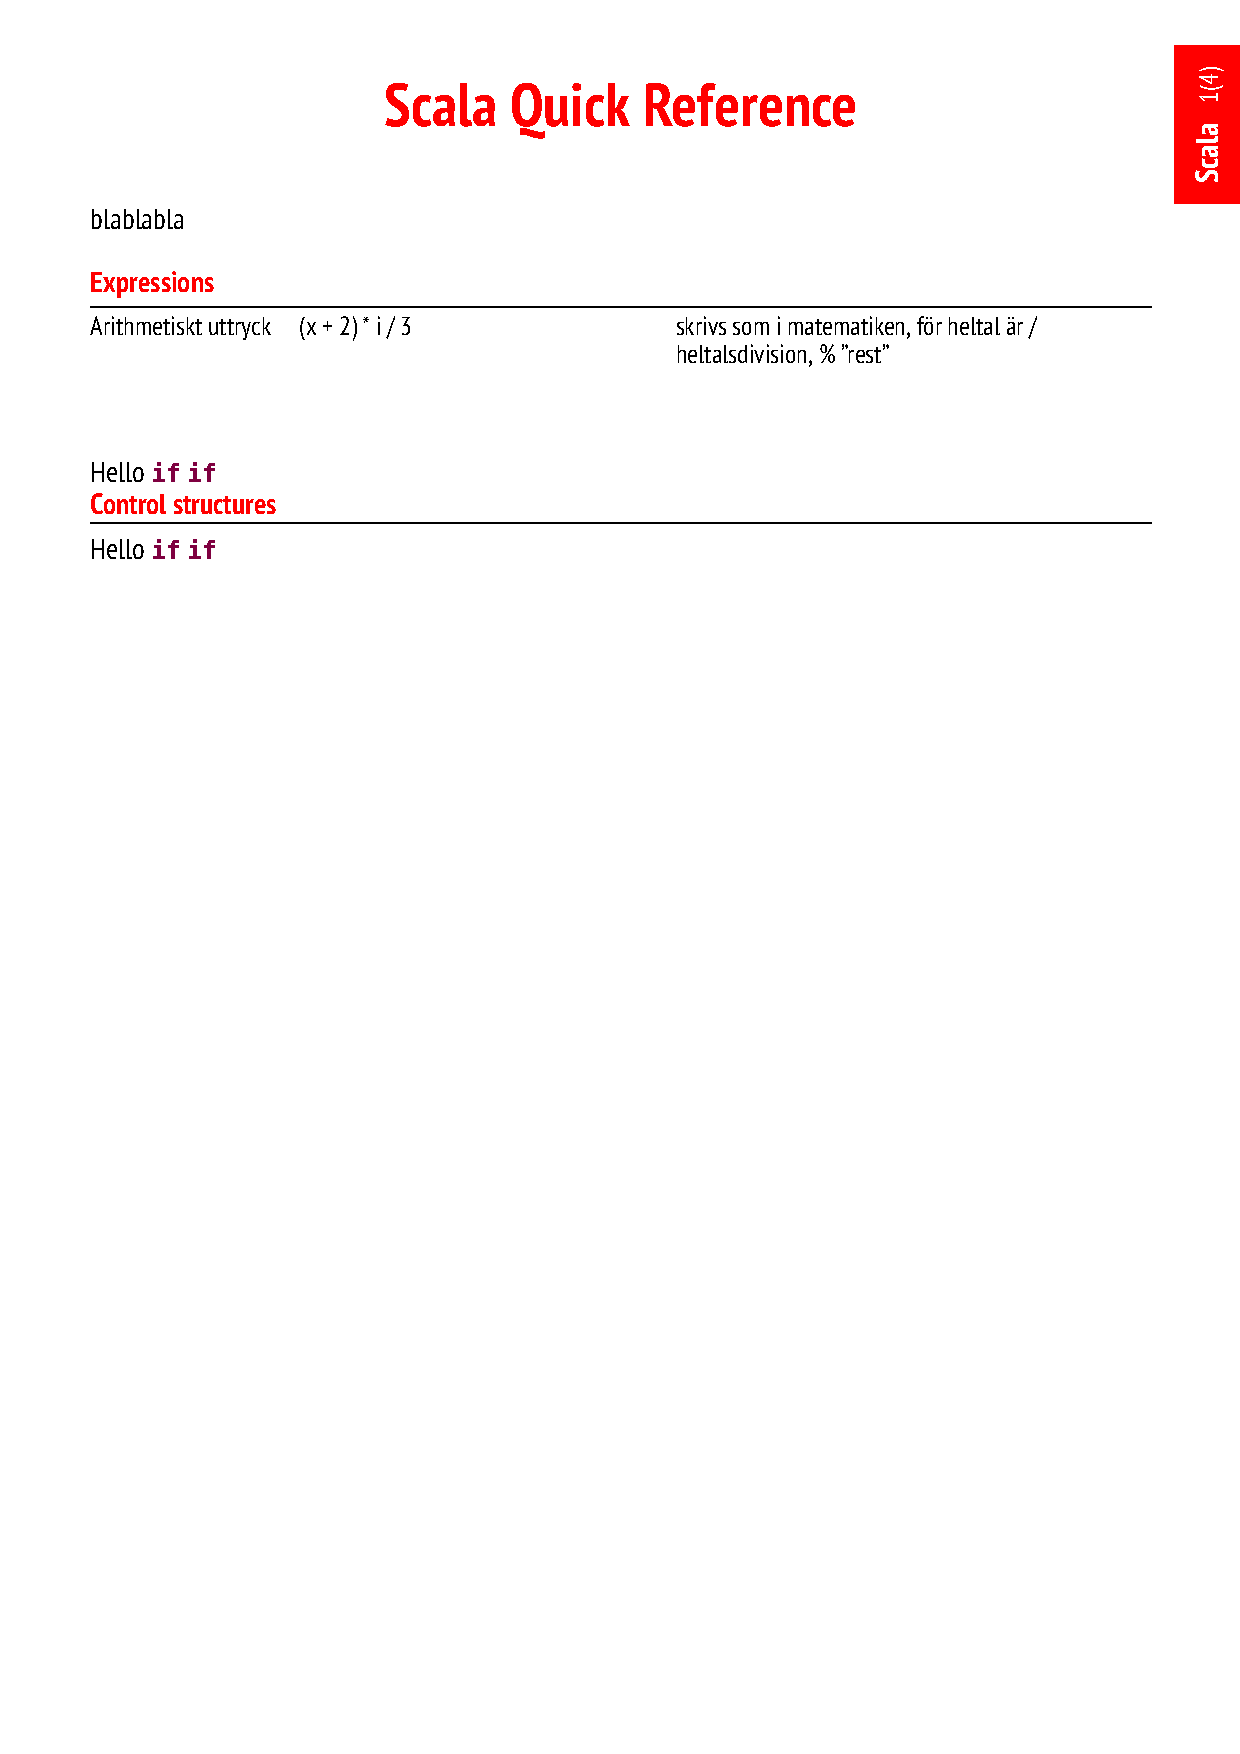
\includepdf[pages={1-12}, scale=0.77, frame]{../quickref/quickref.pdf}


\end{document}
